\documentclass[12pt,a4paper]{article}
\usepackage{blindtext}\usepackage{accsupp}

\usepackage{amssymb}
\usepackage{wasysym}
\usepackage{mathrsfs}
\usepackage[utf8]{inputenc}
\usepackage{physics} % Assuming you resolved the package conflicts
\usepackage{anyfontsize}
\usepackage{amsmath,mathtools}
\usepackage{amssymb}
\usepackage{mathrsfs}
\usepackage[margin=0.65in]{geometry}
\usepackage{xcolor}
\usepackage{fancyhdr}
\usepackage{amsfonts}
\usepackage[euler]{textgreek}
\usepackage{chemformula}
\usepackage{titlesec} % For customizing section heading sizes
\usepackage{indentfirst} % For indenting the first paragraph of each section
\usepackage[hidelinks]{hyperref} 
\usepackage{tabularx}
\usepackage{graphicx}
\usepackage{array}
\usepackage{listings}
\usepackage{xcolor}
\usepackage{pdfpages}
\usepackage{booktabs}
\usepackage{enumitem}
% Custom headers and footers using fancyhdr package
\pagestyle{fancy}
\fancyhead[L]{\footnotesize INP-UGA ENES3 M2 SGB}
\fancyhead[R]{\footnotesize New Sustainable Technoglogies}
\fancyhead[C]{\footnotesize 2024 - 2025}
\renewcommand{\headrulewidth}{0.5pt}
\renewcommand{\footrulewidth}{0.5pt}
\fancyfoot[R]{\textcolor{black}{\footnotesize SARY MONYCHOT \& NIANG BORA}}
\fancyfoot[L]{\footnotesize}

% Set up table formatting
\setlength{\arrayrulewidth}{0.5mm}
\setlength{\tabcolsep}{15pt}
\renewcommand{\arraystretch}{0.95}

% Custom command for electron representation

\newcolumntype{C}{>{\centering\arraybackslash}X}
% Customize section heading sizes
\titleformat{\section}{\normalfont\large\Roman{\bfseries}}{\thesection}{1em}{}
\titleformat{\subsection}{\normalfont\normalsize\bfseries}{\thesubsection}{0.75em}{}
\titleformat{\subsubsection}{\normalfont\normalsize\bfseries}{\thesubsubsection}{0.5em}{}

% Customize equation numbering to include section number
\numberwithin{equation}{section}
\lstset{ 
	language=Python,                 % the language of the code
	basicstyle=\ttfamily\footnotesize, % the size of the fonts that are used for the code
	numbers=left,                   % where to put the line-numbers
	numberstyle=\tiny\color{gray},  % the style that is used for the line-numbers
	stepnumber=1,                   % the step between two line-numbers. If it's 1, each line will be numbered
	numbersep=5pt,                  % how far the line-numbers are from the code
	backgroundcolor=\color{white},      % choose the background color. You must add \usepackage{color}
	showspaces=false,               % show spaces adding particular underscores
	showstringspaces=false,         % underline spaces within strings
	showtabs=false,                 % show tabs within strings adding particular underscores
	frame=single,                   % adds a frame around the code
	rulecolor=\color{black},        % if not set, the frame-color may be changed on line-breaks within not-black text (e.g. comments (green here))
	tabsize=4,                      % sets default tabsize to 2 spaces
	captionpos=b,                   % sets the caption-position to bottom
	breaklines=true,                % sets automatic line breaking
	breakatwhitespace=false,        % sets if automatic breaks should only happen at whitespace
	keywordstyle=\color{blue},      % keyword style
	commentstyle=\color{green},   % comment style
	stringstyle=\color{red},      % string literal style
}

\begin{document}
	\title{\textbf{PEM Fuel Cell system analysis }}
	\author{SARY Monychot \& NIANG Bora }
	%\date{\today}
	\maketitle
		% Table of Contents
	\tableofcontents
% =============================================================	
		\newpage
%% =======================================1 . =========================================
	% Sections and Subsections
	\section{\underline{Calculation of the power demand inside the vechicle}}
	\begin{itemize}
	 \item The specification of the vehicle are the following:
	
	\begin{itemize}
		\item  Weight $M = 2000 kg$
		\item Front area $A = 2.25  m^2$
		\item Drag coefficient (or air penetration coefficient) $C = 0.29$ 
		\item Rolling Resistance coefficient $C_r = 0.0115$
		
	\end{itemize}
	
	\item The efforts applied on the vehicle in the rolling direction have to following expression:
	
	\begin{itemize}
		\item Air penetration : 
		\begin{equation}
				F{(t)} = \frac{1}{2}\rho_{air}v^2_{(t)}CA  \label{eq1}
		\end{equation} with $\rho_{air} = 1.2    kg/m^3$
		\item Rolling resistance :	
		\begin{equation}
			 F(t) = MgC_r\cos{\alpha} \label{eq2}
		\end{equation}with $g = 9.81 m/s^2$ and $\alpha$ the slope angle
		\item Climbing or descent : 
		\begin{equation}
			F(t) = Mg\sin{\alpha} \label{eq3}
		\end{equation} 
		
	\end{itemize}
	\end{itemize}
	
	
%% ======================================= a . =========================================	

	\subsection{Calculate and plot the instant power provided by the vechicle powertrain for the road cycles " WLTC " }
	
	$\star$ Consider a flat road $(\alpha = 0)$
	\begin{figure}[htbp]
		\centering
		\begin{tabular}{c @{\qquad} c}
			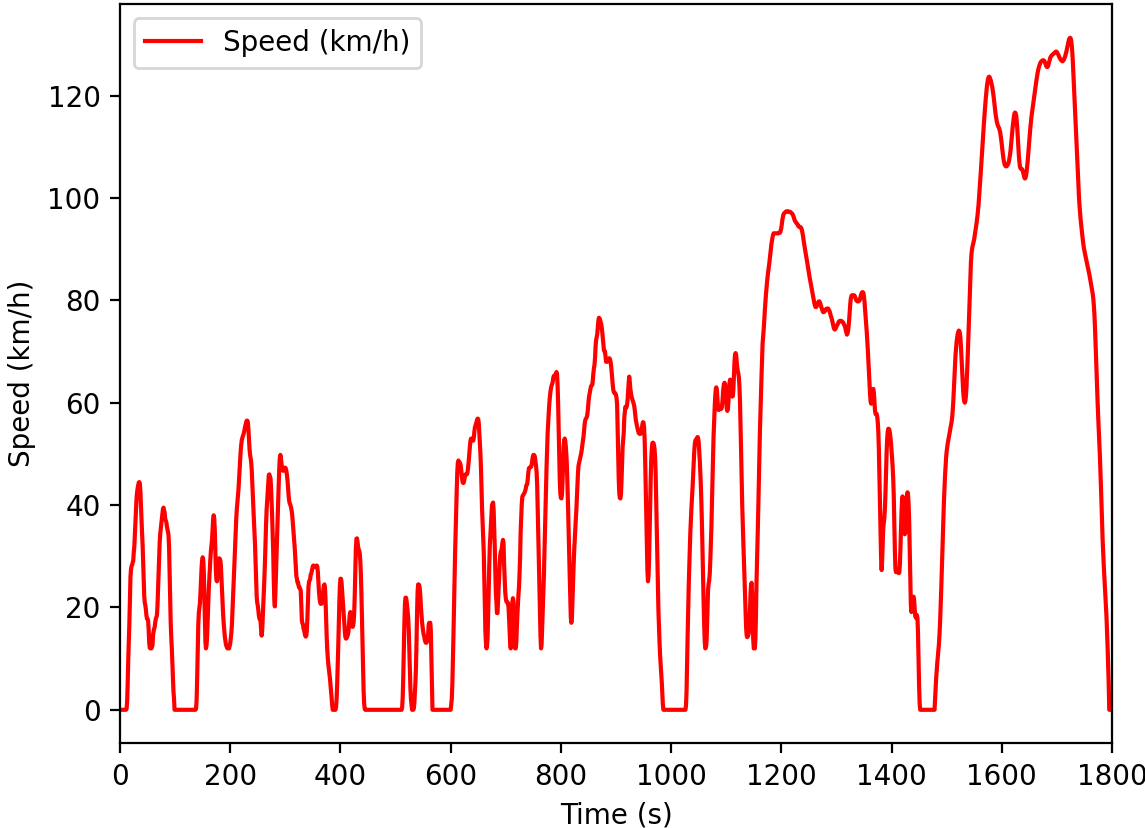
\includegraphics[width=0.48\linewidth]{E:/07. Master_Degree_ITC+UGA/02. ENES3_SGB_UGA/02. New Technology/PEMFC/Speed_1.png} &
			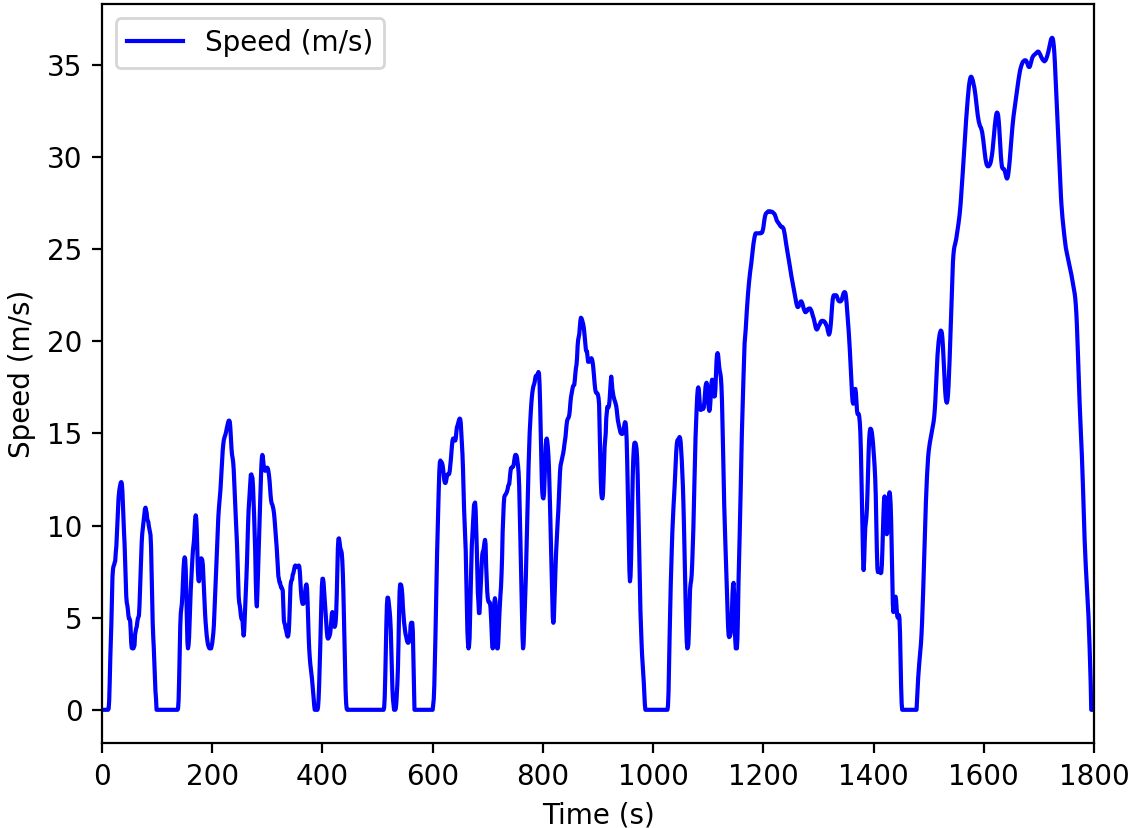
\includegraphics[width=0.48\linewidth]{E:/07. Master_Degree_ITC+UGA/02. ENES3_SGB_UGA/02. New Technology/PEMFC/Speed ms-1_1.png} \\
			
			\small (a) Speed Profile in km/h & \small (b) Speed Profile in m/s
		\end{tabular}
		
		\caption{\small Graph of the Speed Profile in km/h and Speed in m/s}
		\label{1}
	\end{figure}

%% ========================================================================================================
	\subsubsection{Calculation}
	
	To calculate the \textbf{Instant Power}, we need to study of the \textit{force} that have action on the car. By using second Newton's law with the Figure (\ref{2}) shown below, we can assume that there are 4 forces that have action on thecar while driving.
	
	\begin{figure}[h]
		\centering 
		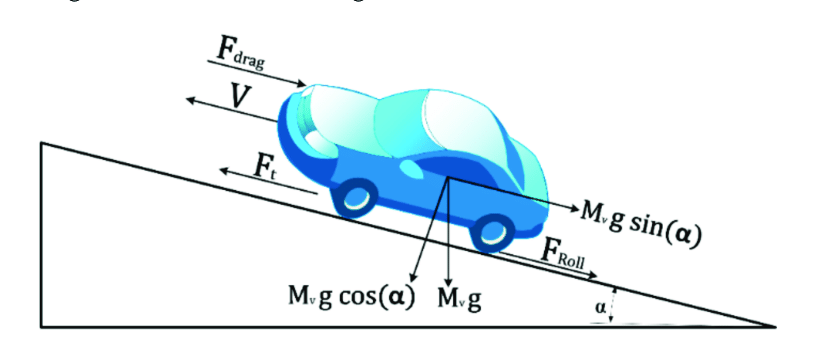
\includegraphics[width=0.7\linewidth]{E:/07. Master_Degree_ITC+UGA/02. ENES3_SGB_UGA/02. New Technology/PEMFC/2.png}
		\caption{\small {Speed (km/h) of the vechicle powertrain by time (s)}}
		\label{2}
	\end{figure}



	\begin{itemize}
		\item The first force is to make the car move in direction. It called the force from motor or machine of the car ($F_{motor}$)
		\item The second force is the rolling force from the car wheels. It called \textbf{Rolling Resistance} ($F_{rolling}$)
		\item The third force is the climbing or descent force ($F_{climb}$)
		\item The fourth force is the force from the air friction. we can called it Air penetration ($F_{air}$).
	\end{itemize}


	Using second Newton's law, we can written :
	\begin{equation}
		\overrightarrow{F}_{motor} - \overrightarrow{F}_{rolling} -\overrightarrow{F}_{climb} - \overrightarrow{F}_{air} = m\overrightarrow{a}
		\label{eq4}
	\end{equation}
	\begin{equation}
		\overrightarrow{F}_{motor} = \overrightarrow{F}_{rolling} + \overrightarrow{F}_{climb} + \overrightarrow{F}_{air} + m\overrightarrow{a}
		\label{eq5}
	\end{equation}

	since $a$ is the acceleration of the vechical in time $t$, as we written : 
	\begin{equation}
		\overrightarrow{a} = \derivative{\overrightarrow{v}}{t} = \frac{\Delta v}{\Delta t}
		\label{eq6}
	\end{equation}

	By using Equation (\ref{eq6}), we can get the result of acceleration on the Figure (\ref{3})
	\begin{figure}[h]
		\centering 
		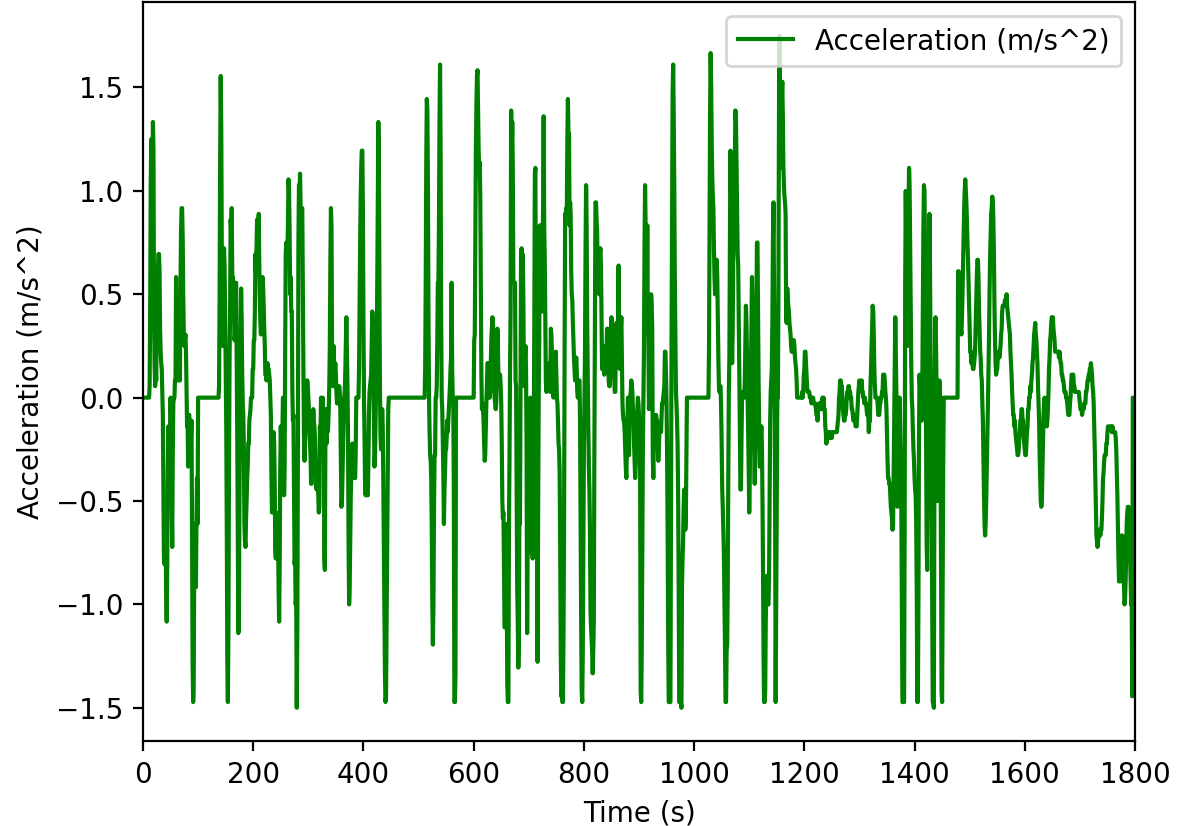
\includegraphics[width=0.65\linewidth]{E:/07. Master_Degree_ITC+UGA/02. ENES3_SGB_UGA/02. New Technology/PEMFC/Acceleration_1.png}
		\caption{\small {Acceleration $(m/s^2)$ of the vechicle powertrain by time (s)}}
		\label{3}
	\end{figure}

	According to the graph, it shown that the vechical did not have the stable speed drive on the. At the some time ($t$), the vechical increasing the speed immediately. In contrast, at some time ($t$), the vechical reducing the speed quickly as shown in the Figure (\ref{3}).

	\begin{itemize}[label=-]
		\item For calculate $F_{air}$ by using Equation (\ref{eq1}) , we got :
			\begin{equation}




				F_{air}(t) = \frac{1}{2}\rho_{air}v^2CA = \frac{1}{2}\times1.2\times 	v^2_{m/s}_{,t}\times0.29\times 		2.25 \label{eq7}
			\end{equation}
			In this section, to calculate $F_{air}$ we need to get the speed in each time $t$ in $m/s^2$ to analyze in the Equation (\ref{eq7})
			By using the Equation (\ref{eq1}), we got the result of the force air penetration by shown in below graph.
		\item For calculate $F_{rolling}$, we will be using the Equation (\ref{eq2}), we got :
			\begin{equation}
				F_{rolling}(t) = MgC_r\cos(\alpha) = 2000kg\times9.81m/s^2\times0.0115\times\cos(0^\circ) = \textbf{225.630} \label{eq8}
			\end{equation}
			For this force, it will be constant in time $(t)$ becuase there is not any parameter in the Equation (\ref{eq8}) will change in which time.
			
			
		\item For calculate $F_{climb}$, we will use Equation (\ref{eq4}) then we got:
		
			\begin{equation}
				F_{climb}(t) = Mg\sin(\alpha) = 2000kg \times 9.81m/s^2 \times \sin(0^\circ) = 0 \label{eq9}
			\end{equation}		
	\end{itemize}

	By using Equation (\ref{eq6}), (\ref{eq7}), (\ref{eq8}) and (\ref{eq9}) substitution into Equation (\ref{eq5}). The result of total force was shown by the graph in Figure (\ref{4}).
	
	\begin{figure}[htbp]
		\centering
		\begin{tabular}{c @{\qquad} c}
			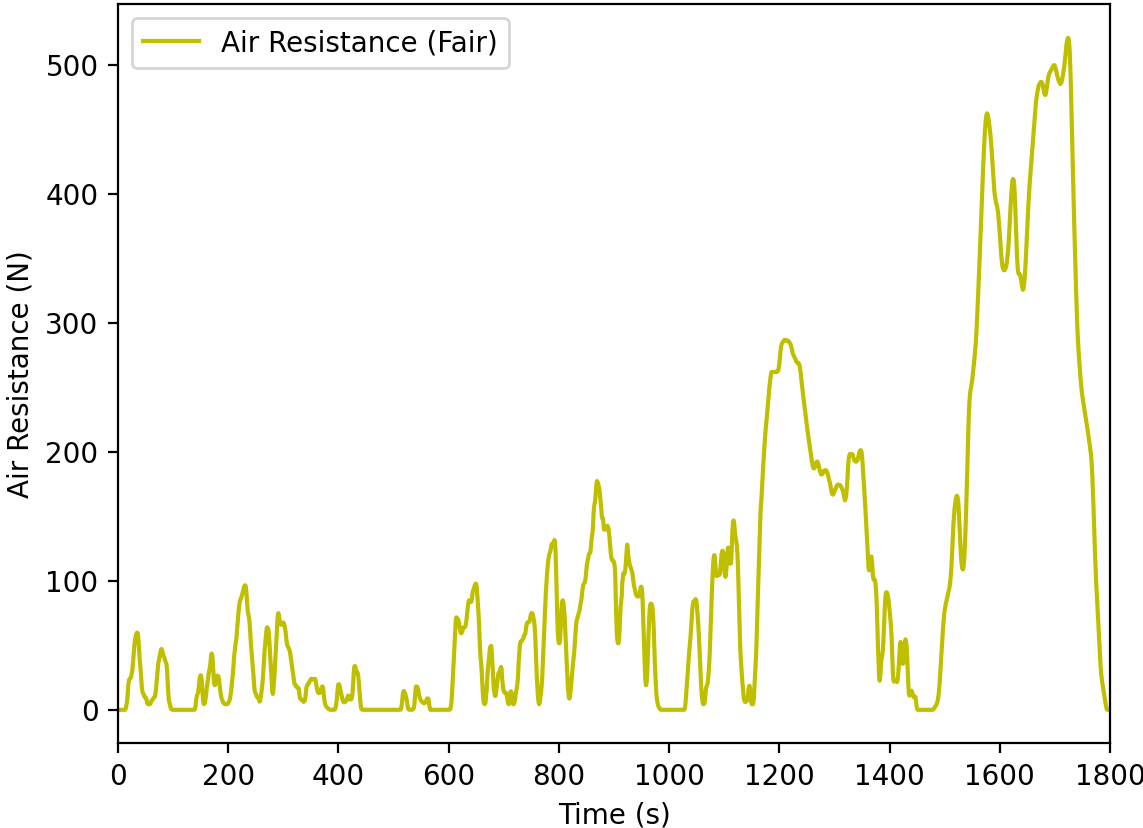
\includegraphics[width=0.48\linewidth]{E:/07. Master_Degree_ITC+UGA/02. ENES3_SGB_UGA/02. New Technology/PEMFC/Fair_1.png} &
			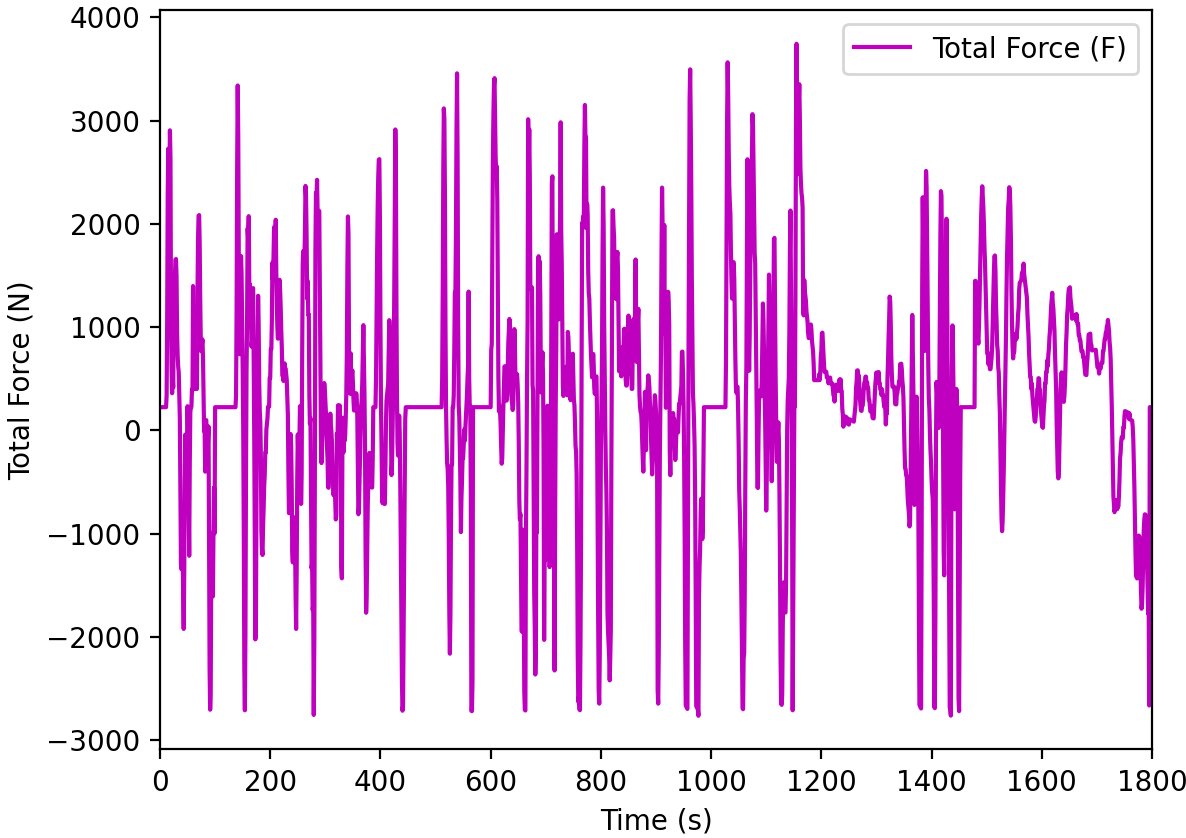
\includegraphics[width=0.48\linewidth]{E:/07. Master_Degree_ITC+UGA/02. ENES3_SGB_UGA/02. New Technology/PEMFC/Total_Force_1.png} \\
			
			\small (a) Force of Air Resistance & \small (b) Total Force
		\end{tabular}
		
		\caption{\small Graph of the  Force of Air Resistance and Total Force}
		\label{4}
	\end{figure}
		
	To calculate Instant power we are using :
	
	\begin{equation}
		P = F \times v \label{eq10}
	\end{equation}	
	
	The result of the instant power calcuation will be show at Figure (\ref{5})b. The instant power of the vechical are depend on two parameter :
	\begin{itemize}
		\item The total force from the vechical action ($N$).
		\item The speed that make the vechical go forward ($m/s$).
	\end{itemize}	                                                                                                                                                                  
	\indent As now, we can write that 
		\begin{equation}
			P_t = F_t \times v_t 
		\end{equation} 
	\newpage
	
	 The result of the instant power will show in the Figure ({\ref{5}).
	 
	 \begin{figure}[h]
	 	\centering 
	 	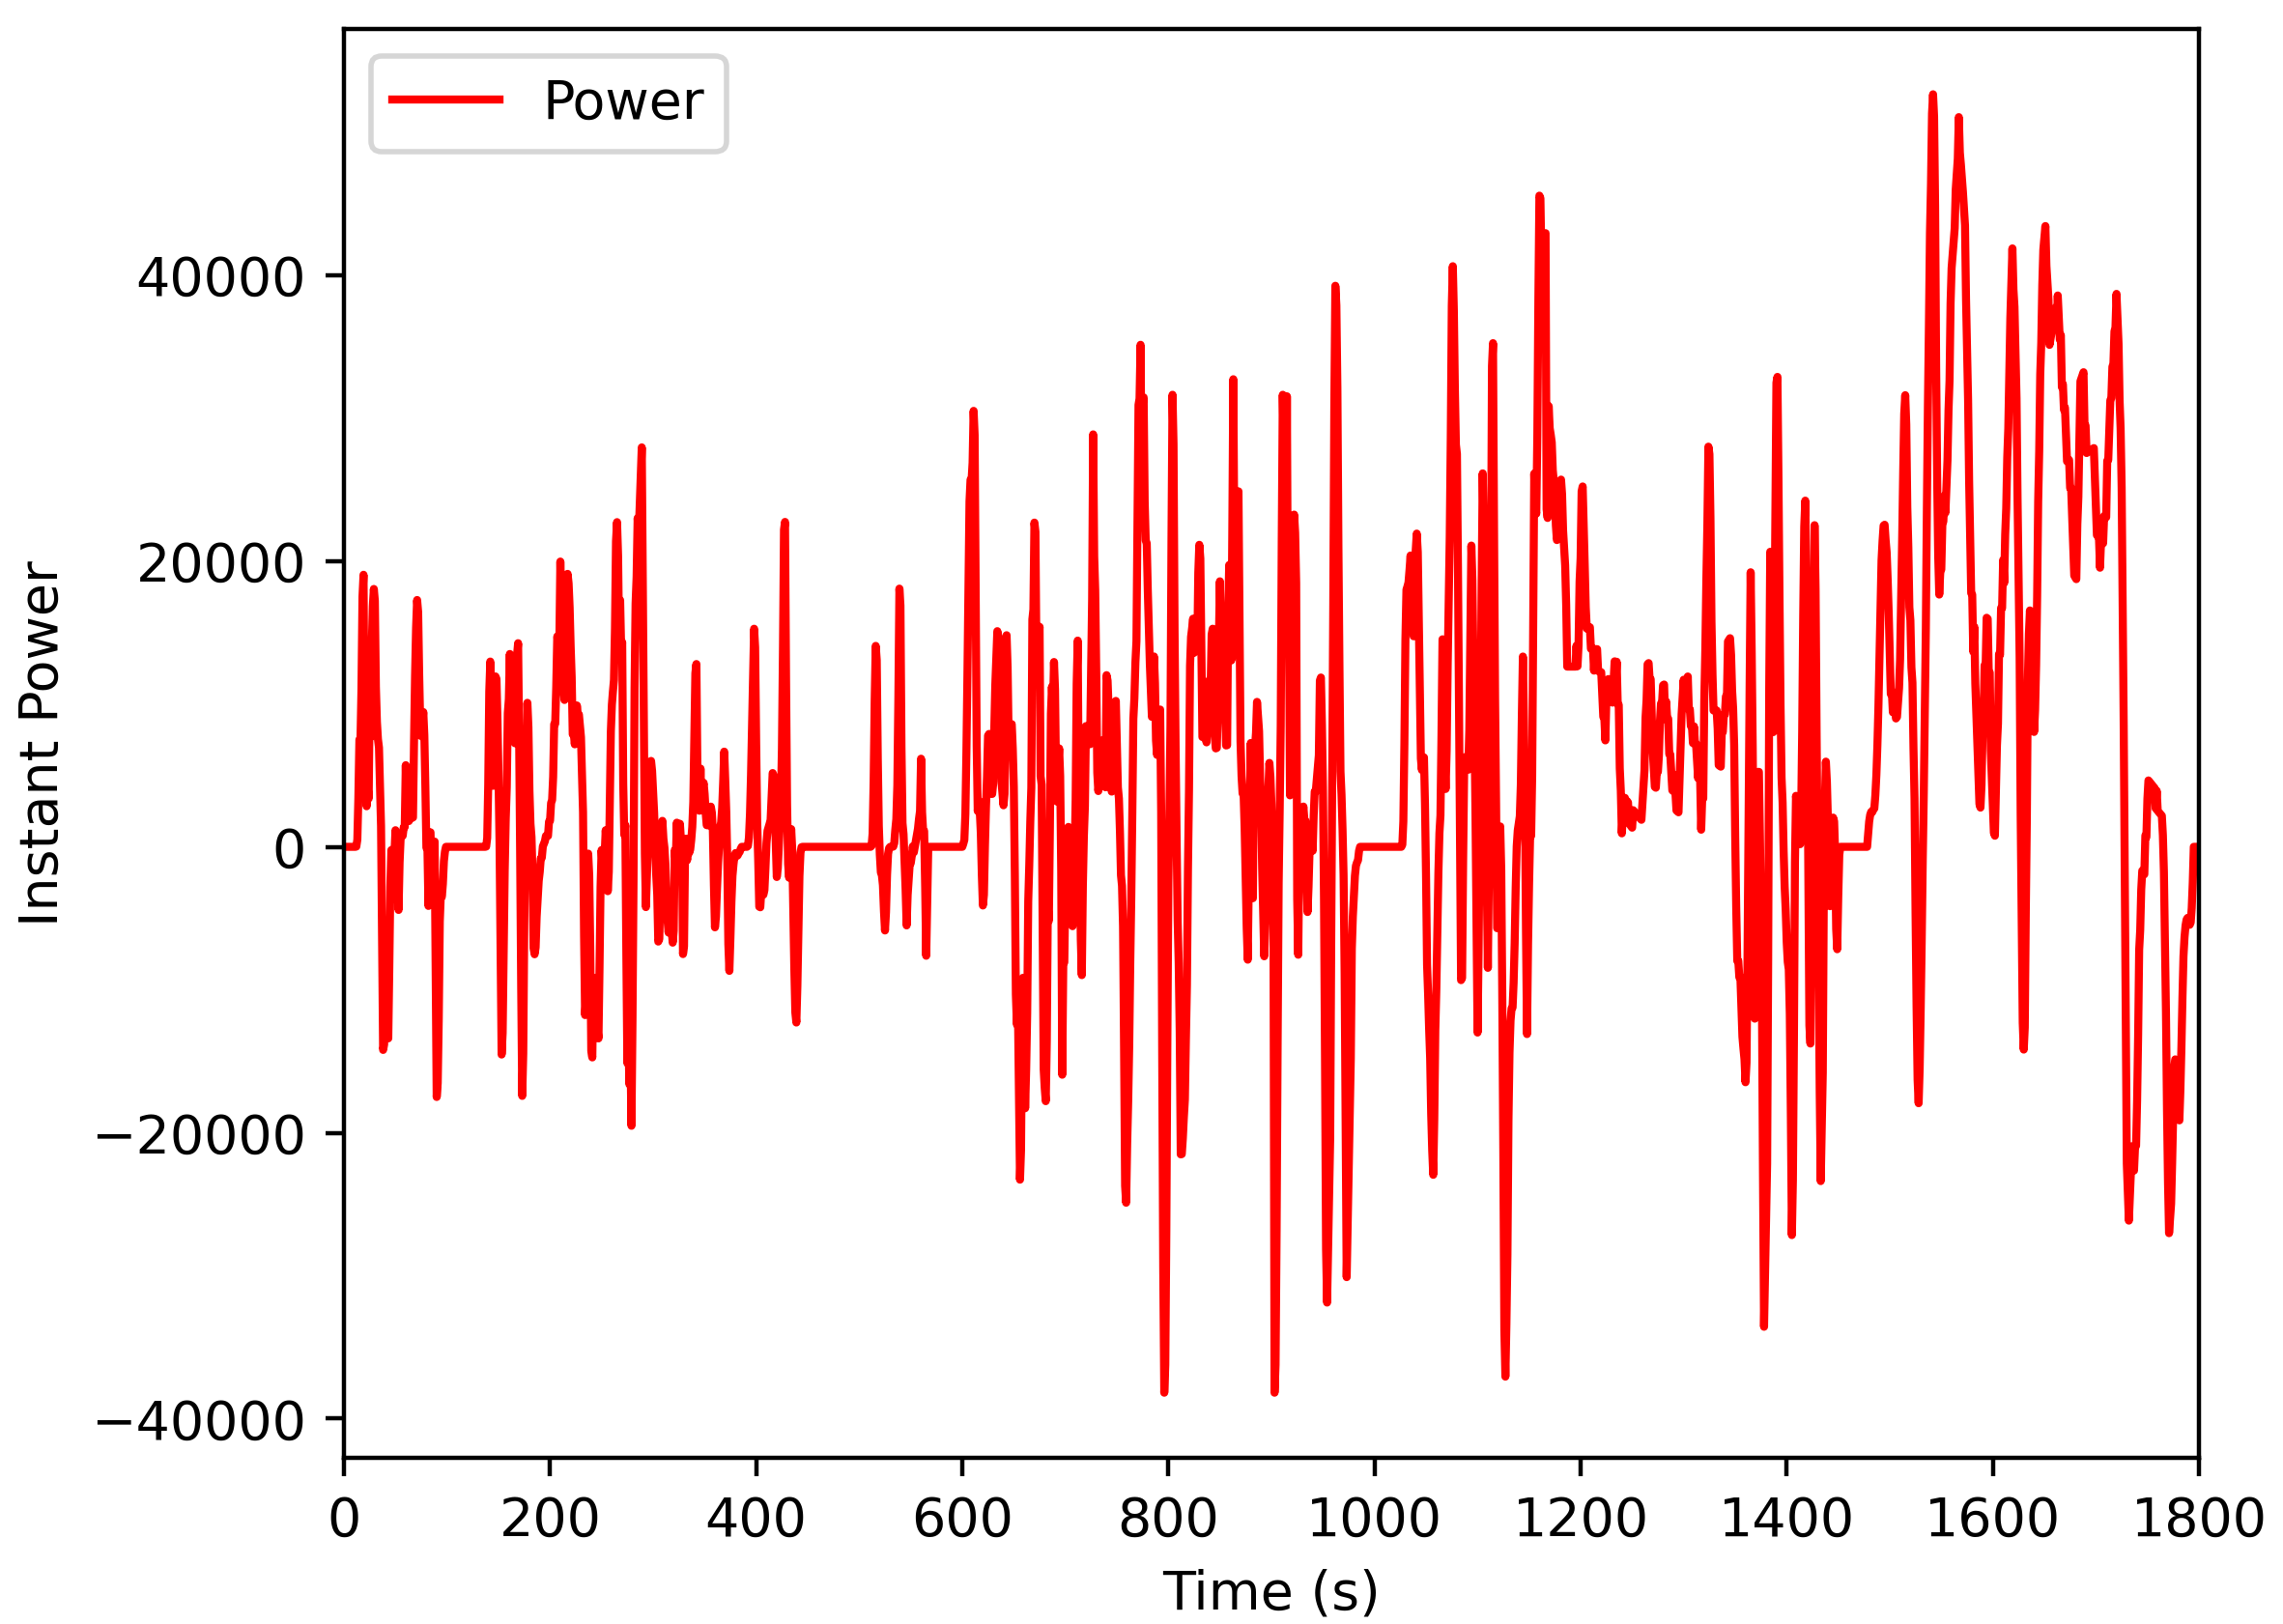
\includegraphics[width=0.7\linewidth]{E:/07. Master_Degree_ITC+UGA/02. ENES3_SGB_UGA/02. New Technology/PEMFC/Power_1.png}
	 	\caption{\small {Instant Power of the Vechicle (W)}}
	 	\label{5}
	 \end{figure}
	
%% ======================================= b . =========================================

	\subsection{Calculate the instant power provide (positive) or received (negative) by the electric hybrid power source. }
	
	The vehicle auxiliaries consume an electrical power of 300W (no air conditioning, minimum consumption of all the equipment of the vehicle: sensor, supervisor,etc.) The DC/DC converter efficiency is assumed constant at 90\% both direction.
	
	\begin{figure}[h]
		\centering 
		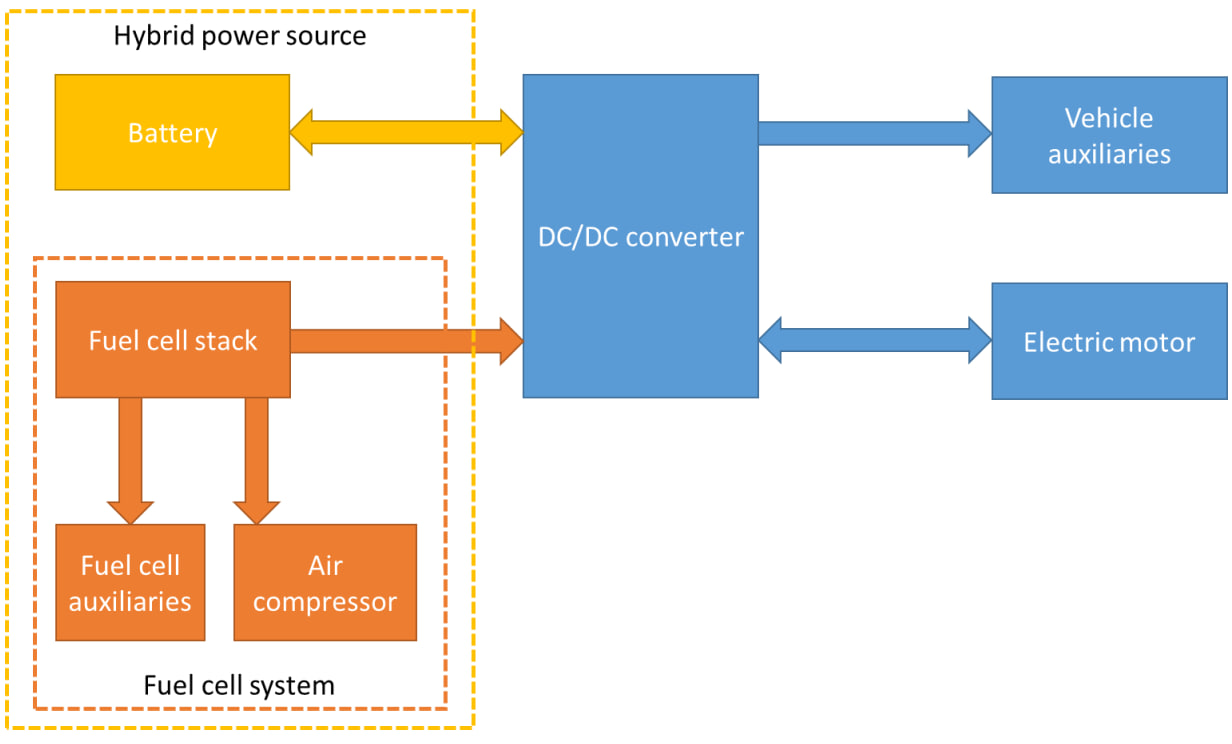
\includegraphics[width=0.8\linewidth]{E:/07. Master_Degree_ITC+UGA/02. ENES3_SGB_UGA/02. New Technology/PEMFC/DC.jpg}
		\caption{\small {Hybrid system in the vehicle}}
		\label{6}
	\end{figure}
\newpage
	\begin{figure}[h]
		\centering 
		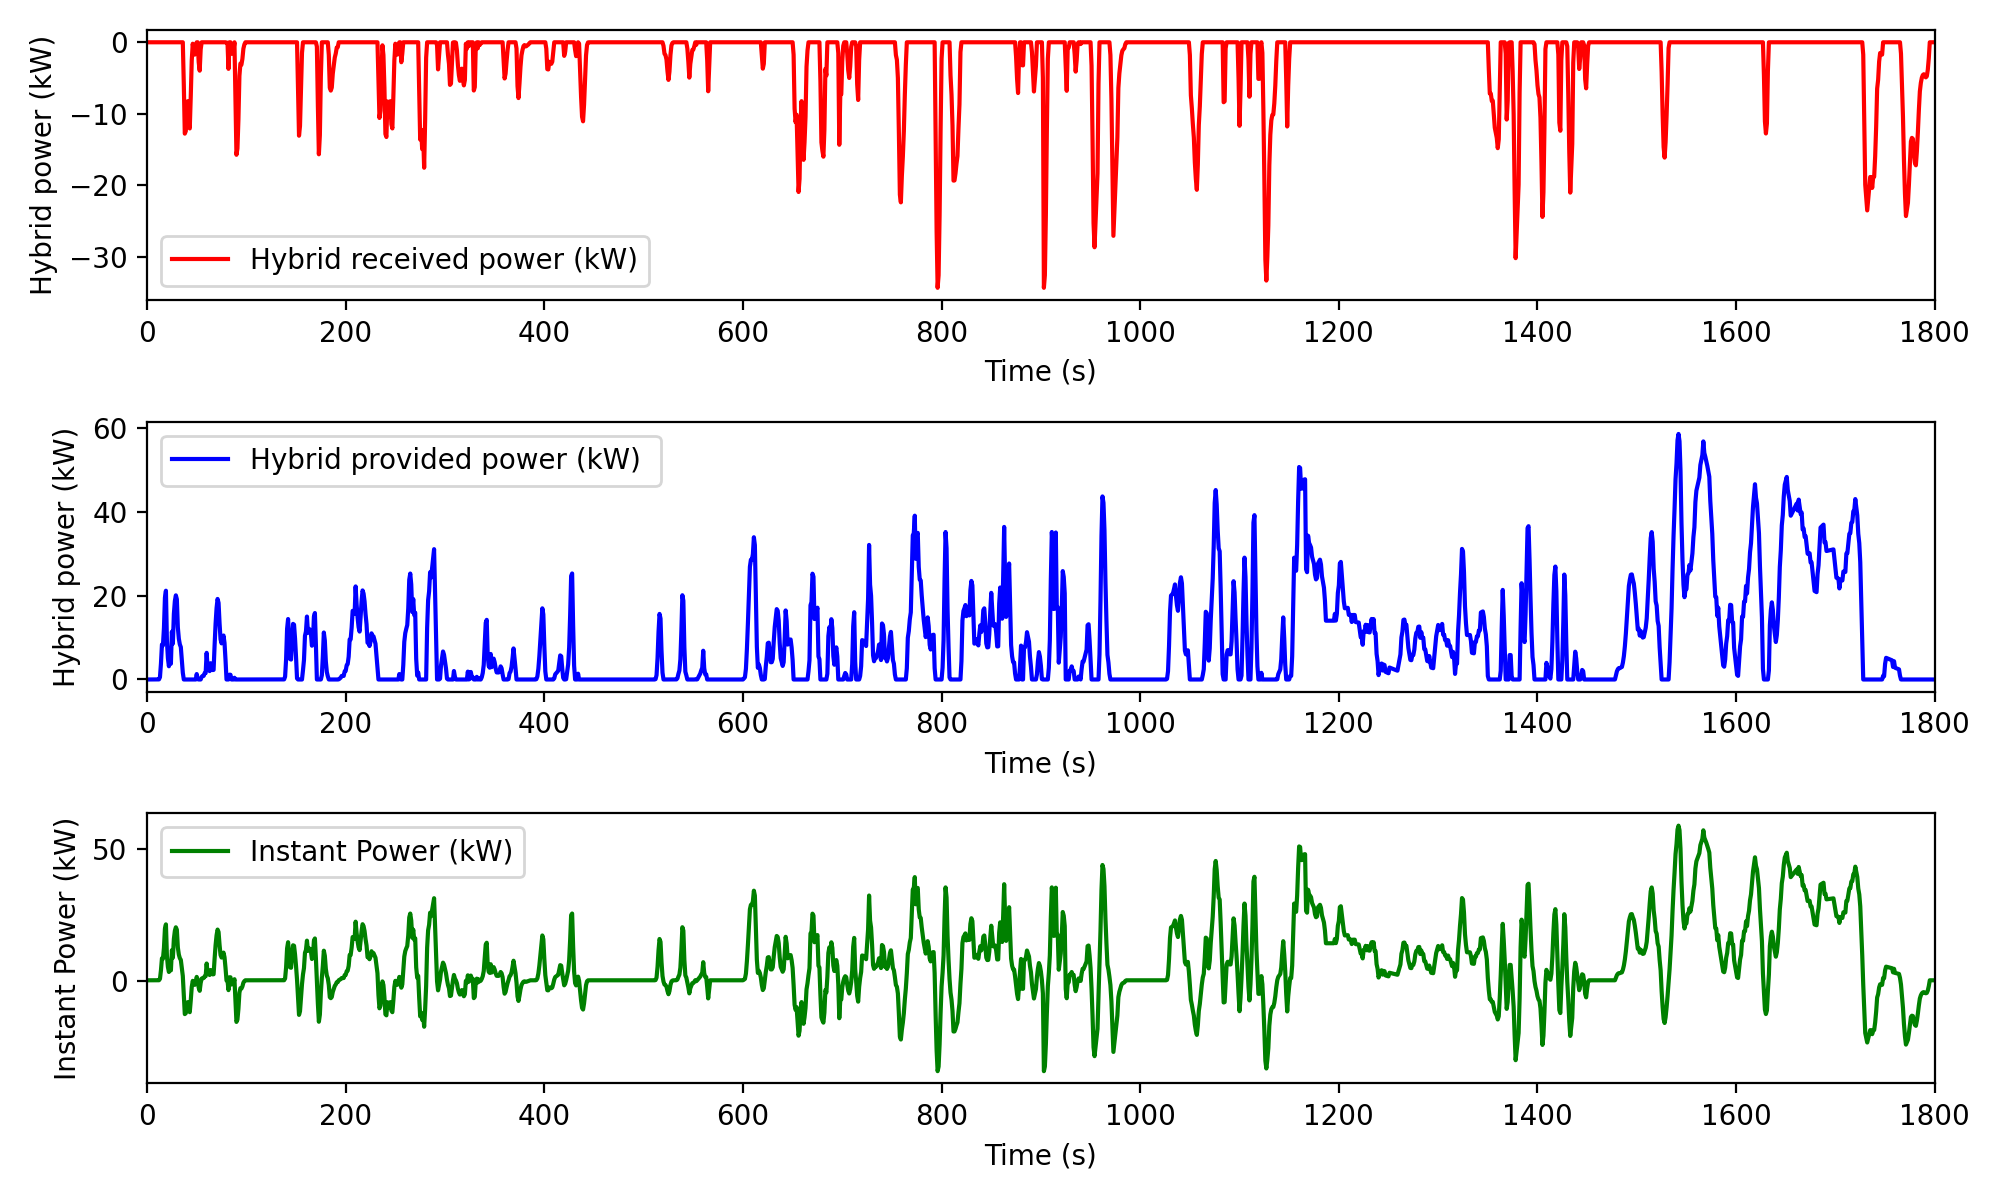
\includegraphics[width=0.95\linewidth]{E:/07. Master_Degree_ITC+UGA/02. ENES3_SGB_UGA/02. New Technology/PEMFC/Question_B.png}
		\caption{\small {Hybrid working system in power transfer}}
		\label{7}
	\end{figure}
	To find the transfer power in the hybrid system in order to find the provided (positive) or recevied (negative), we have use instant power from pervious question as data in the Figure (\ref{5}) with the efficieny of the DC/DC converter. As shown in the Figure (\ref{7}): At the \textbf{first figure} had been show the \textbf{RED line graph} represented the received power (negative) to the hybrid power with the maximum received is \textbf{34.365 kW}. Moreover, as shown in the \textbf{second figure} shown the \textbf{Blue line graph} represented the provided power (positive) from the hybrid system to the motor and auxiliaries. The maximum provided power to the motor was around \textbf{58.488 kW}. According to data from the calculation, we can assumed that the vechicle mostly consum power from the hybrid and less provided power to hybrid system based on the data of speed that provided. 
	
	
	
	
	
	
%% ======================================= c . =========================================





\subsection{Calculate and Plot as a function of time : The power of the battery (kW), The power of the fuel cell system (kW), The SOC battery (\%) }	

The energy management strategy of the hybridization between the battery and the fuel cell system is not disclosed by Tooyta. 
\begin{itemize}
	\item The battery technology is Li-ion, with a stored energy of \textbf{1.24kWh}.
	\item The test results of Mirai 1 indicate that the battery State of Charge (SoC) is comprised between \textbf{50\%} and \textbf{65\%}
	\item The power delivered by the battery is often close to \textbf{5\%} of the total power provided by the hybrid power source when $SoC < 55\%$ or \textbf{30\%} when $SoC > 55\%$
	\item Discharging power of the battery is approximately \textbf{12.4 kW} (or 10C), while the charging power depends on the battery SoC: \textbf{10C} if $SoC < 55\%$ or \textbf{6C} if $SoC > 55\%$
	\item The battery provides $0\%, 5\%, 30\%$ of the total power depending on its SoC and in the limit of its maximum discharging power.
	\item The EMS avoids values of SoC below 50\% and above 65\%
	\item The fuel cell system provides the rest of the power reuqired, excpet if the power demand is too low: the power provided by the fuel cell system can't be lower than \textbf{2.5kW}
\end{itemize}  

	\begin{figure}[h]
	\centering 
	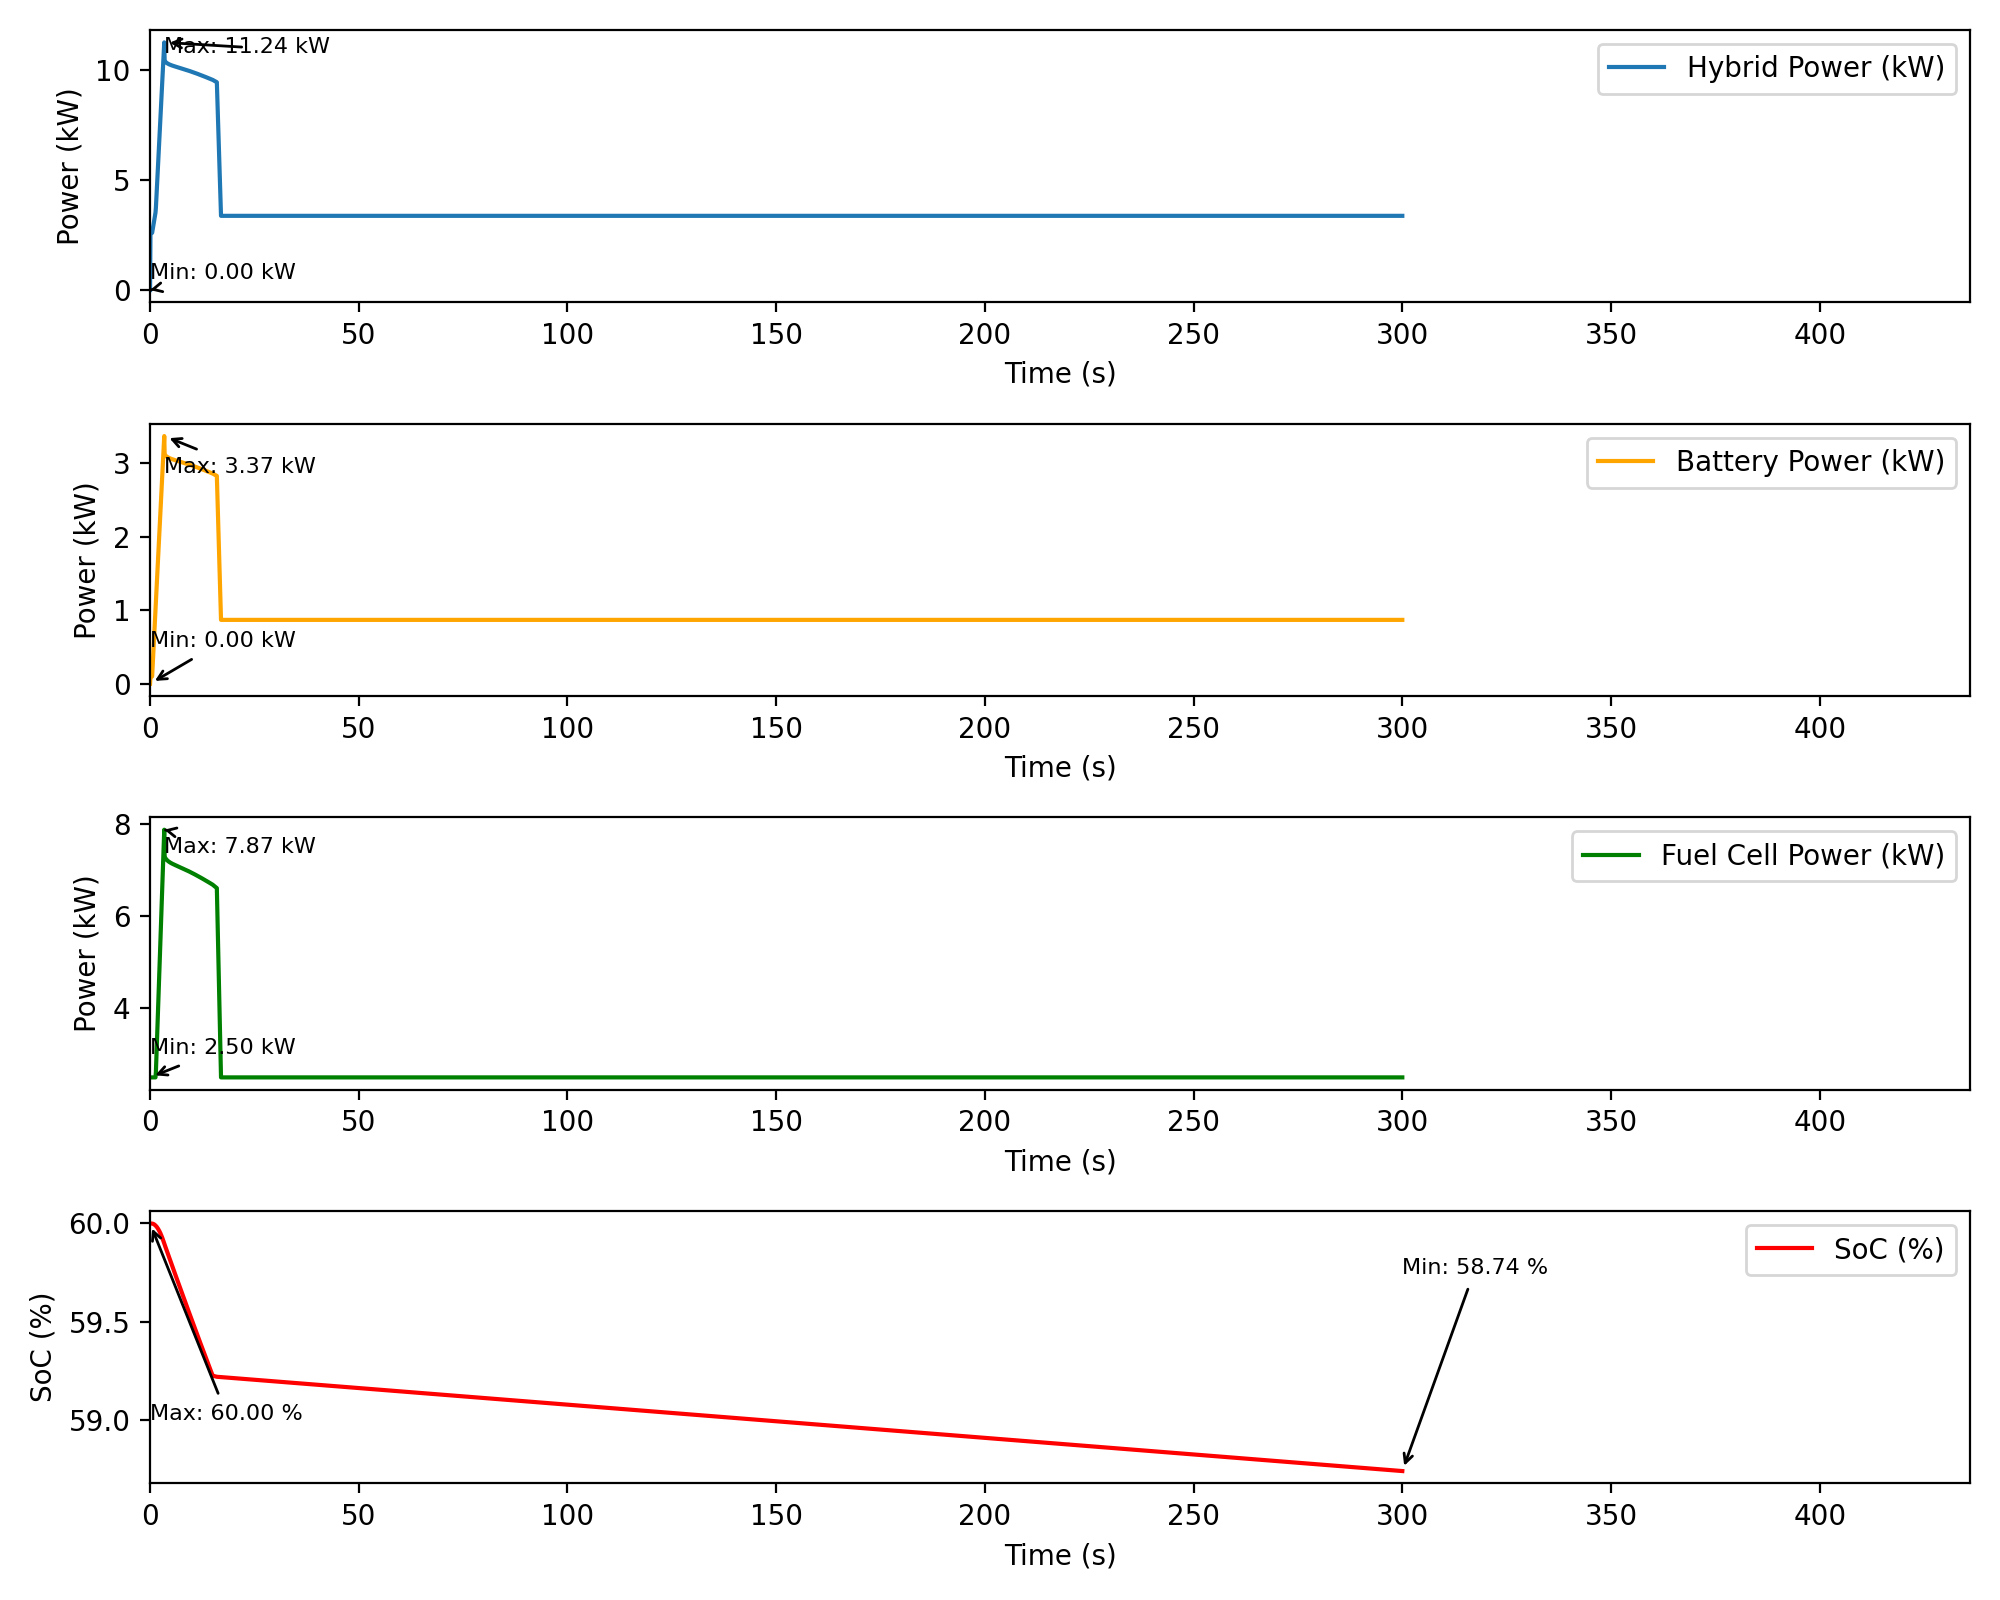
\includegraphics[width=0.95\linewidth]{E:/07. Master_Degree_ITC+UGA/02. ENES3_SGB_UGA/02. New Technology/PEMFC/Question_C.png}
	\caption{\small {Hybrid system, Battery Management, Fuel Cell power and State of Charge in the Vehicle}}
	\label{8}
	\end{figure}

	As the result that shown in the Figure (\ref{8}), 
	\begin{itemize}
		\item The first plot of the Figure (\ref{8}) (represented by the by blue curve) show about the \textbf{Hybrid Power} working in the system.
		\item The second plot of the Figure (\ref{8}) (represented by the by yellow curve) show the characteristic of the charging and discharging of the Battery in the vehicle. The maximum power discharging is \textbf{12.4 kW} and the maximum power charging is \textbf{7.44 kW}. The status of charge and discharge ws depend on the time and speed per second.
		\item  The third plot of the Figure (\ref{8}) (represented by the by green curve) show the fuel cell consumption that will be use in the system. The maximum fuel cell consumption is \textbf{46.42 kW}. The consumption of the fuel cell variable depend on the time.
		\item The fourth plot in Figure (\ref{8}) (represented by the by red curve) illustrates the State of Charge (SoC) of the battery system. By using formula to determine State of Charge in the system, we do it by : 
	\begin{equation}
			\text{SoC}_i = \min\left( \text{SoC}_{\text{max}}, \max\left( \text{SoC}_{\text{min}}, \text{SoC}_{i-1} - \frac{\text{power bat}_i}{3600 \cdot \text{batcapacity}} + \frac{\text{demand}_i}{3600 \cdot \text{batcapacity}} \right) \right)
	\end{equation}

		
		It starts with an initial SoC of approximately \textbf{60\%} and gradually decreases to \textbf{56.28\%} over time, depending on the driving characteristics. The SoC can fluctuate, increasing or decreasing based on the motor's operation and the dynamics of the hybrid system.
		
	\end{itemize}


%% ======================================= d . =========================================

\subsection{Make the same analysis with the road cycle "130 kmh". Consider two different cases : $\alpha = 0^\circ$ and $\alpha = 2^\circ$ } 
	
	\subsubsection{Analysis $\alpha = 0^\circ$}
		\begin{figure}[h]
			\centering 
			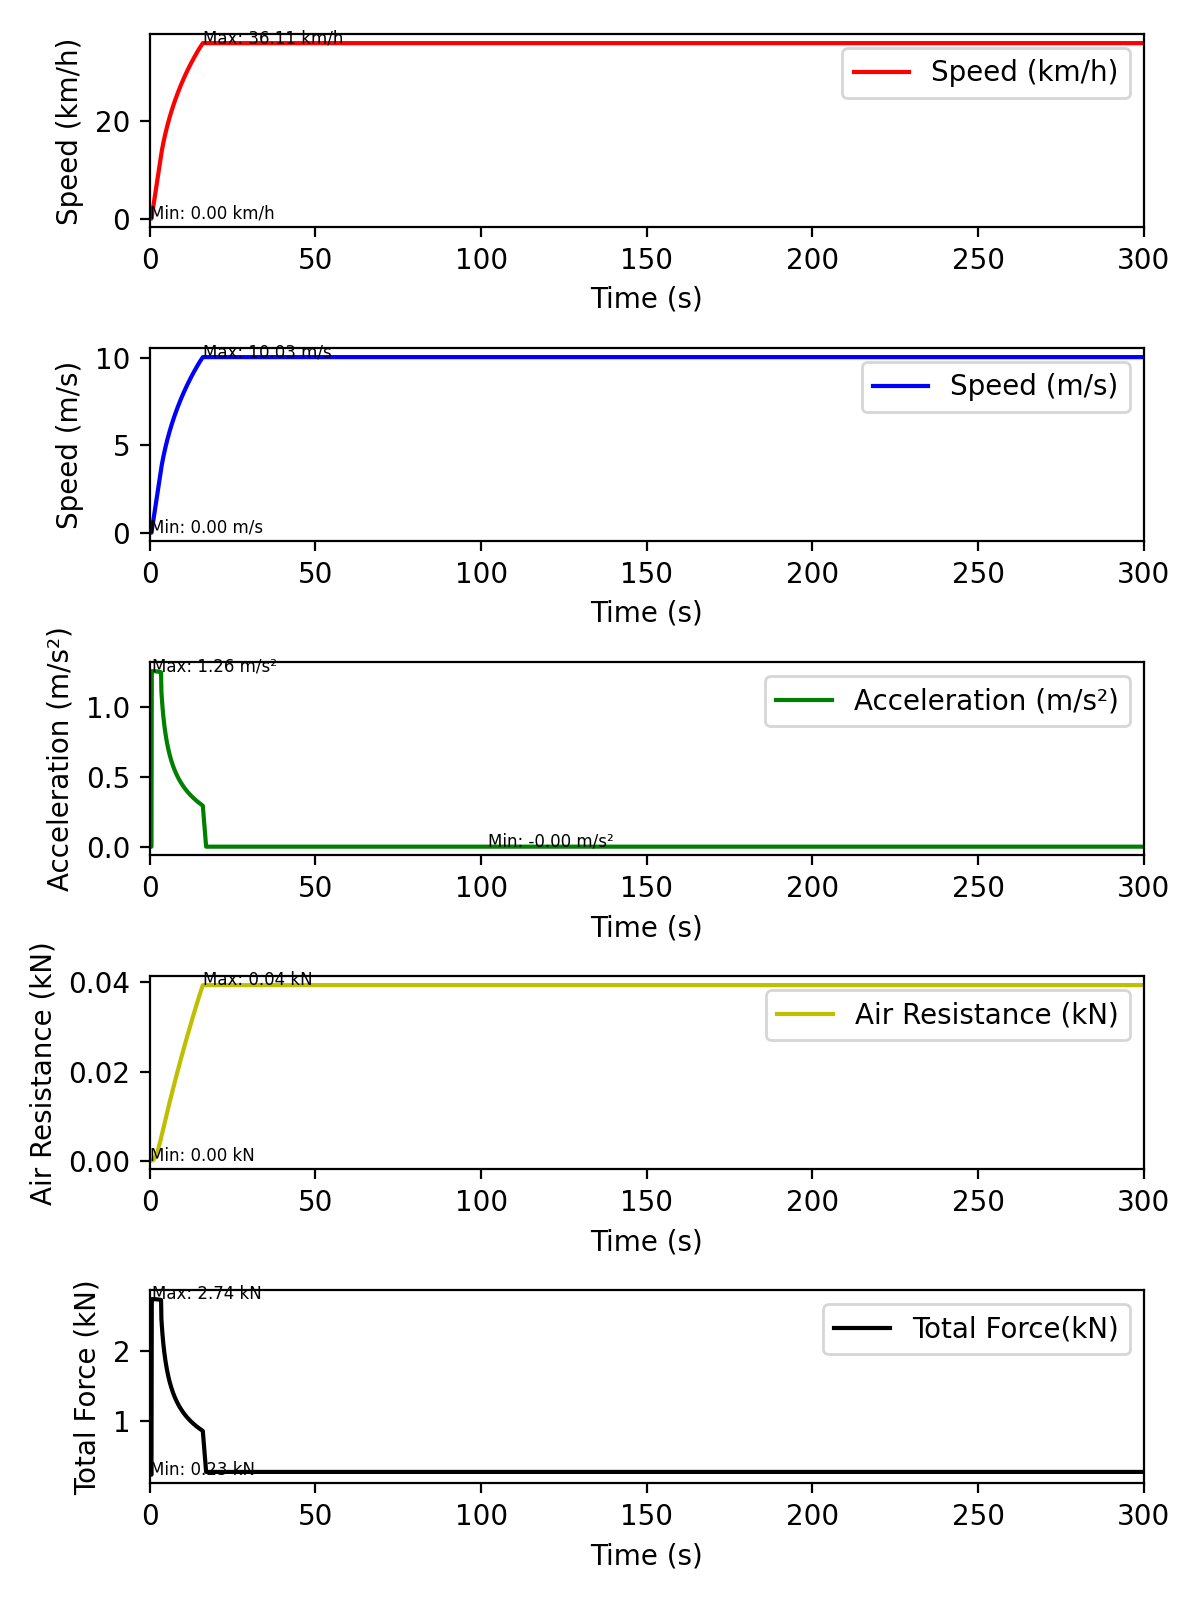
\includegraphics[width=0.83\linewidth]{E:/07. Master_Degree_ITC+UGA/02. ENES3_SGB_UGA/02. New Technology/PEMFC/Question_A_130.png}
			\caption{\small {Plots related to Speed, acceleration, air resistance, and Total Force over time}}
			\label{9}
		\end{figure}

	In the Figure (\ref{9}), it was shown the data curve about the speed within $km/h$ and $m/s$, acceleration in $m/s^2$, Air Resistance and Rolling Resistance.

\begin{itemize}
	\item The first red and blue curve in the Figure (\ref{9}) represented to the speed of the vehicle drive over time in $km/h$ and $m/s$.
	\item The green curve in the Figure (\ref{9}) presented to the acceleration of the vehicle that show the characteristic of the vehicle drive. (Increase or Decrease Speed)
	\item The air resistance calculated by using Equation (\ref{eq1})  and (\ref{eq8}) . The result of the calculate shown in the yellow curve of the Figure (\ref{9}).
	\item The total Force or Motor Force determined by usig Equation (\ref{eq5}) and the result of the calculation displayed at the black curve shown that the maximum motor force is \textbf{2.74 kN}.
\end{itemize}


\begin{figure}[h]
	\centering 
	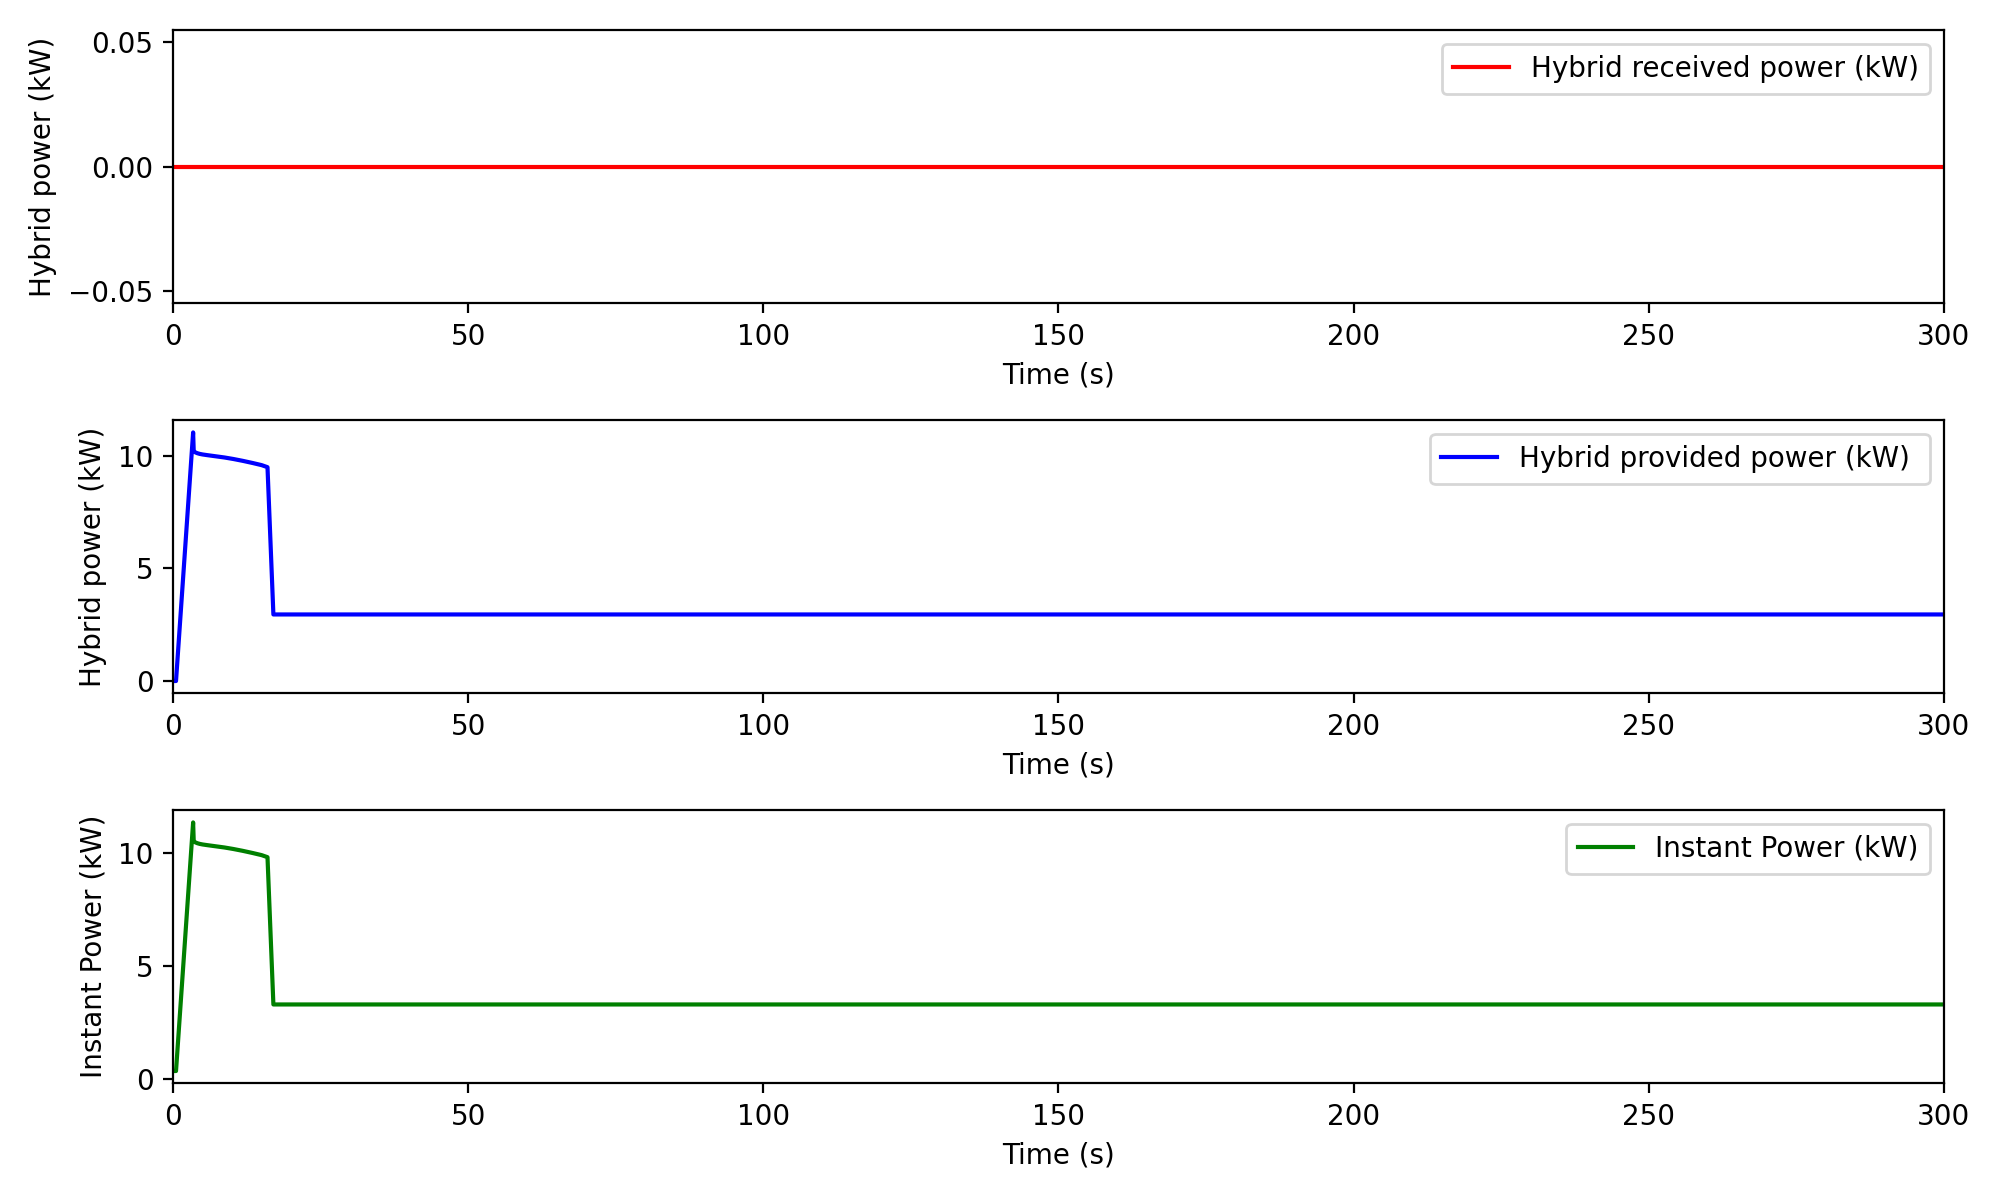
\includegraphics[width=0.9\linewidth]{E:/07. Master_Degree_ITC+UGA/02. ENES3_SGB_UGA/02. New Technology/PEMFC/Question_B_130.png}
	\caption{\small {Hybrid working in Power transfer in Vehicle 130kmh}}
	\label{10}
\end{figure}
As show in Figure (\ref{10}), we can assume that vehicle at this speed characteristic shown that the Hybrid system did not receive any power from the motor but it provided full power to the motor.


\begin{figure}[h]
	\centering 
	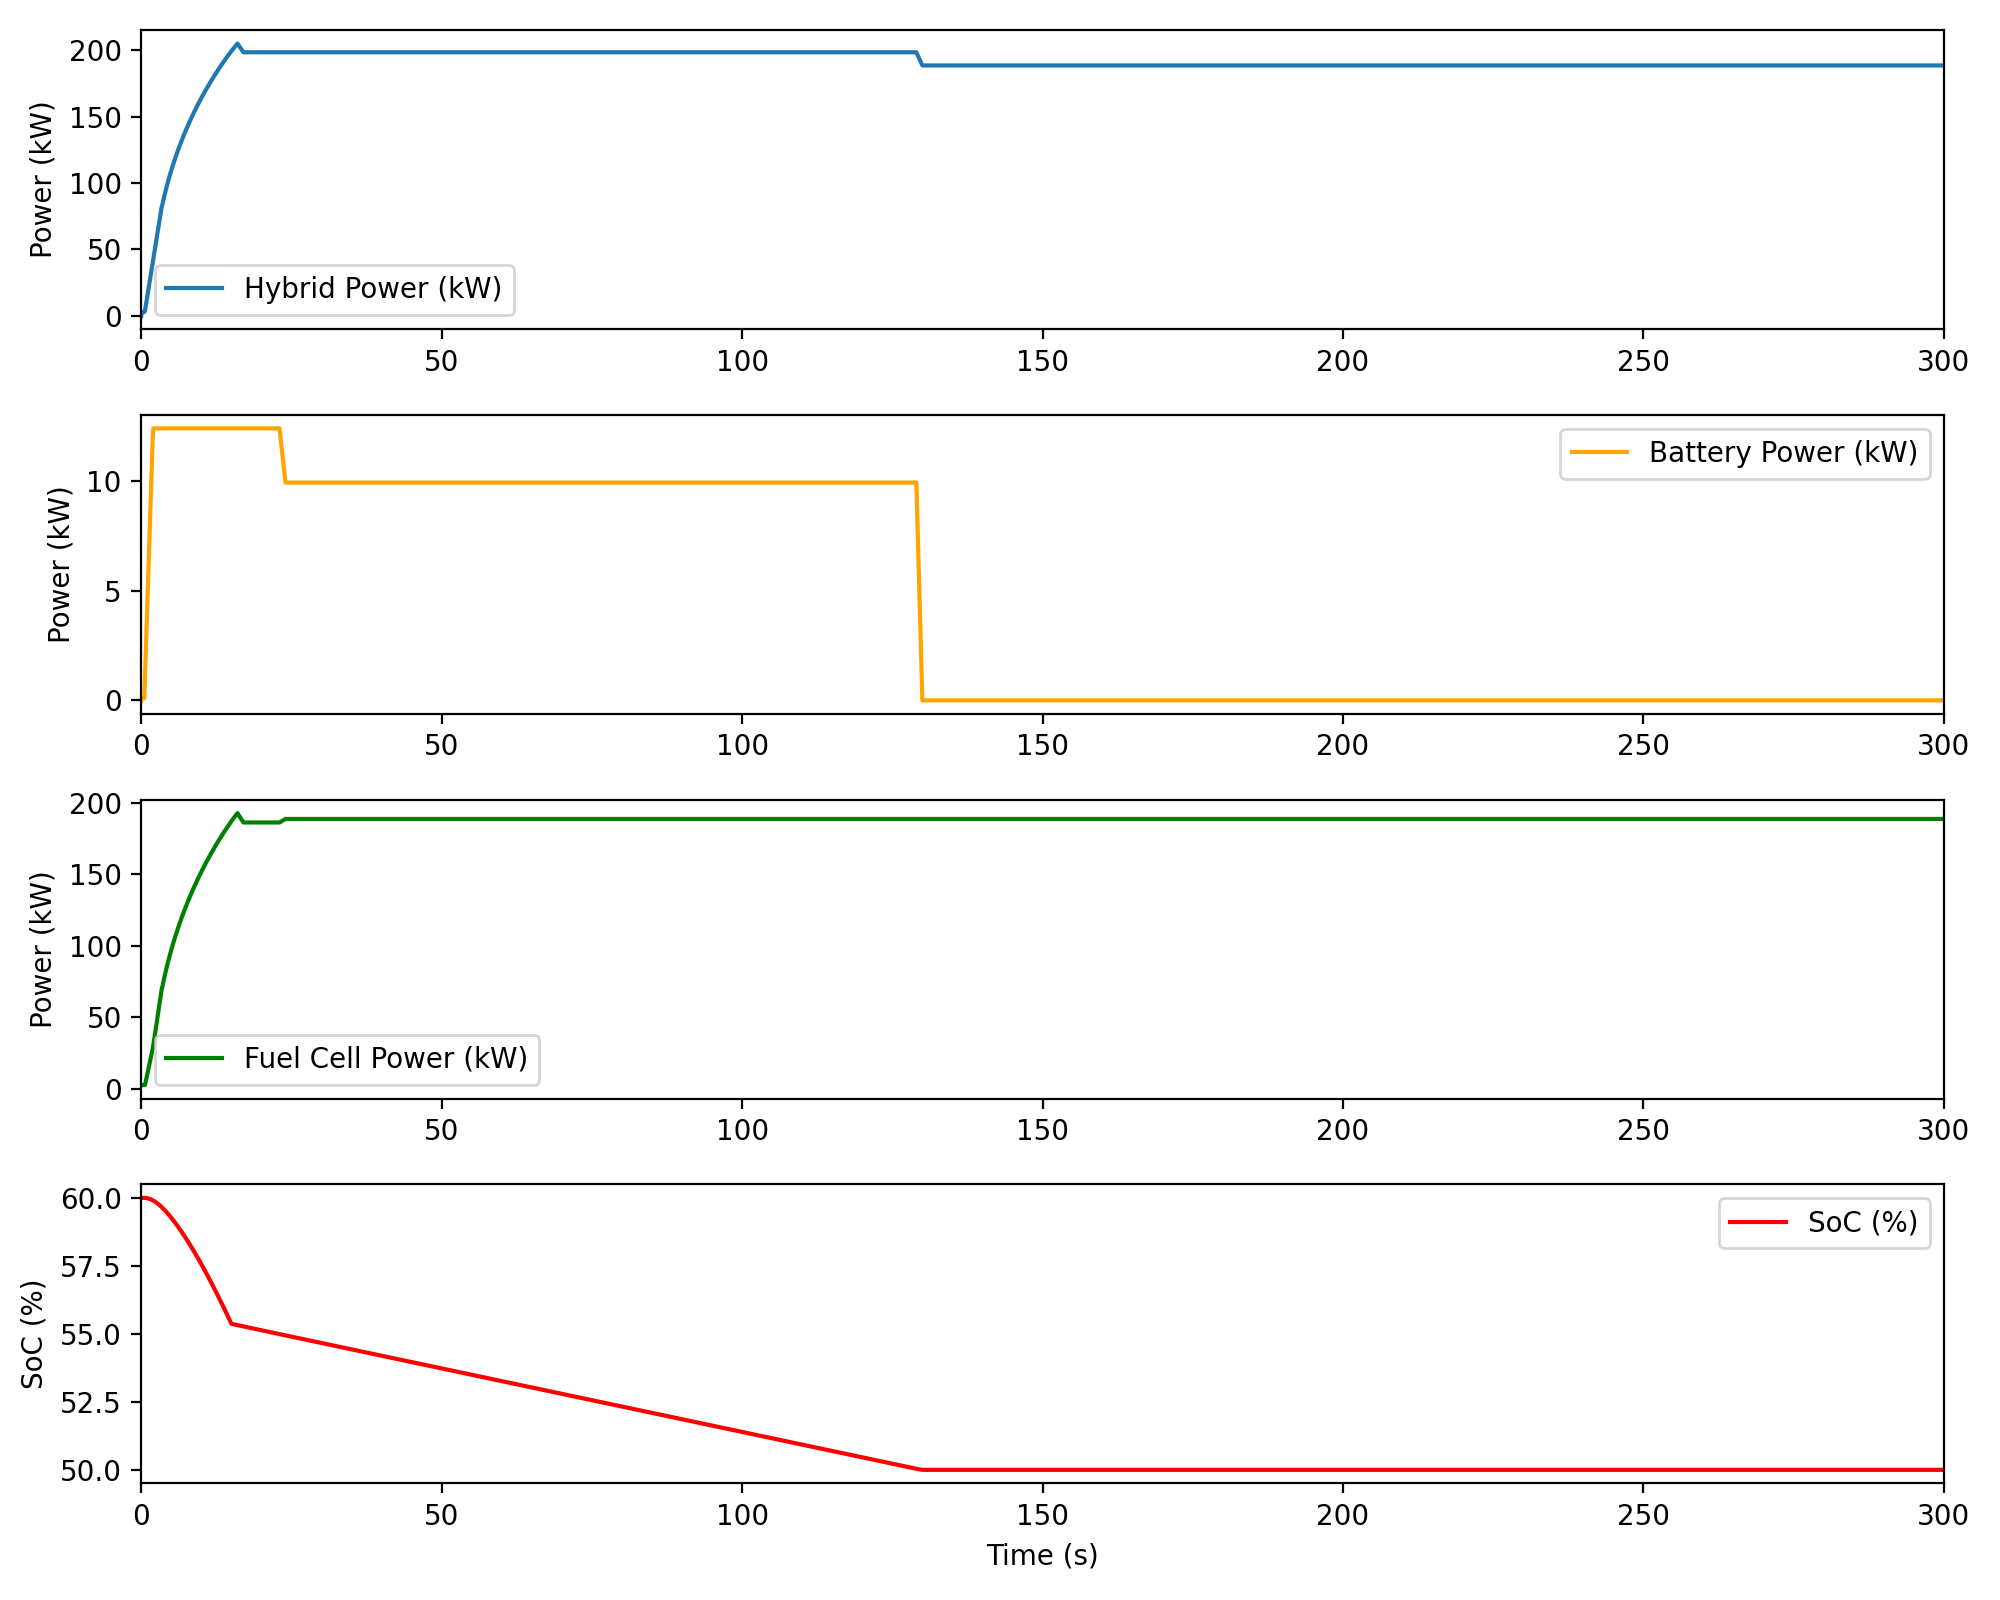
\includegraphics[width=0.9\linewidth]{E:/07. Master_Degree_ITC+UGA/02. ENES3_SGB_UGA/02. New Technology/PEMFC/Question_C_130.png}
	\caption{\small {Hybrid system, Battery Management, Fuel Cell power and State of Charge in the Vehicle}}
	\label{11}
\end{figure}
\begin{itemize}
	\item \textbf{Hybrid Power (kW)}:
	\begin{itemize}
		\item This plot shows the total hybrid power delivered by the system.
		\item The power reaches a peak of approximately 3.17 kW at the start.
		\item It rapidly drops to 0 kW after around 25 seconds and remains flat for the rest of the 300-second period.
	\end{itemize}
	
	\item \textbf{Battery Power (kW)}:
	\begin{itemize}
		\item This plot shows the power supplied by the battery alone.
		\item Initially, the battery power spikes to a peak of around 3.31 kW.
		\item It sharply decreases to 0 kW after about 25 seconds, staying at that level for the rest of the duration.
	\end{itemize}
	
	\item \textbf{Fuel Cell Power (kW)}:
	\begin{itemize}
		\item This plot shows the power generated by the fuel cell.
		\item The fuel cell power reaches a maximum of about 2.76 kW early in the period.
		\item It drops rapidly to 2.5 kW within 25 seconds and remains constant at this level for the remainder of the time.
	\end{itemize}
	
	\item \textbf{State of Charge (SoC) (\%)}:
	\begin{itemize}
		\item This plot represents the battery’s state of charge (SoC) over time.
		\item The SoC starts at approximately 60\% and decreases gradually over time.
		\item By the end of the 300-second period, it reaches around 59.3\%.
	\end{itemize}
\end{itemize}




% ======================================C .  ALPHA 2 =====================================================\\

\subsubsection{Analysis $\alpha = 2^\circ$}


\begin{figure}[h]
	\centering 
	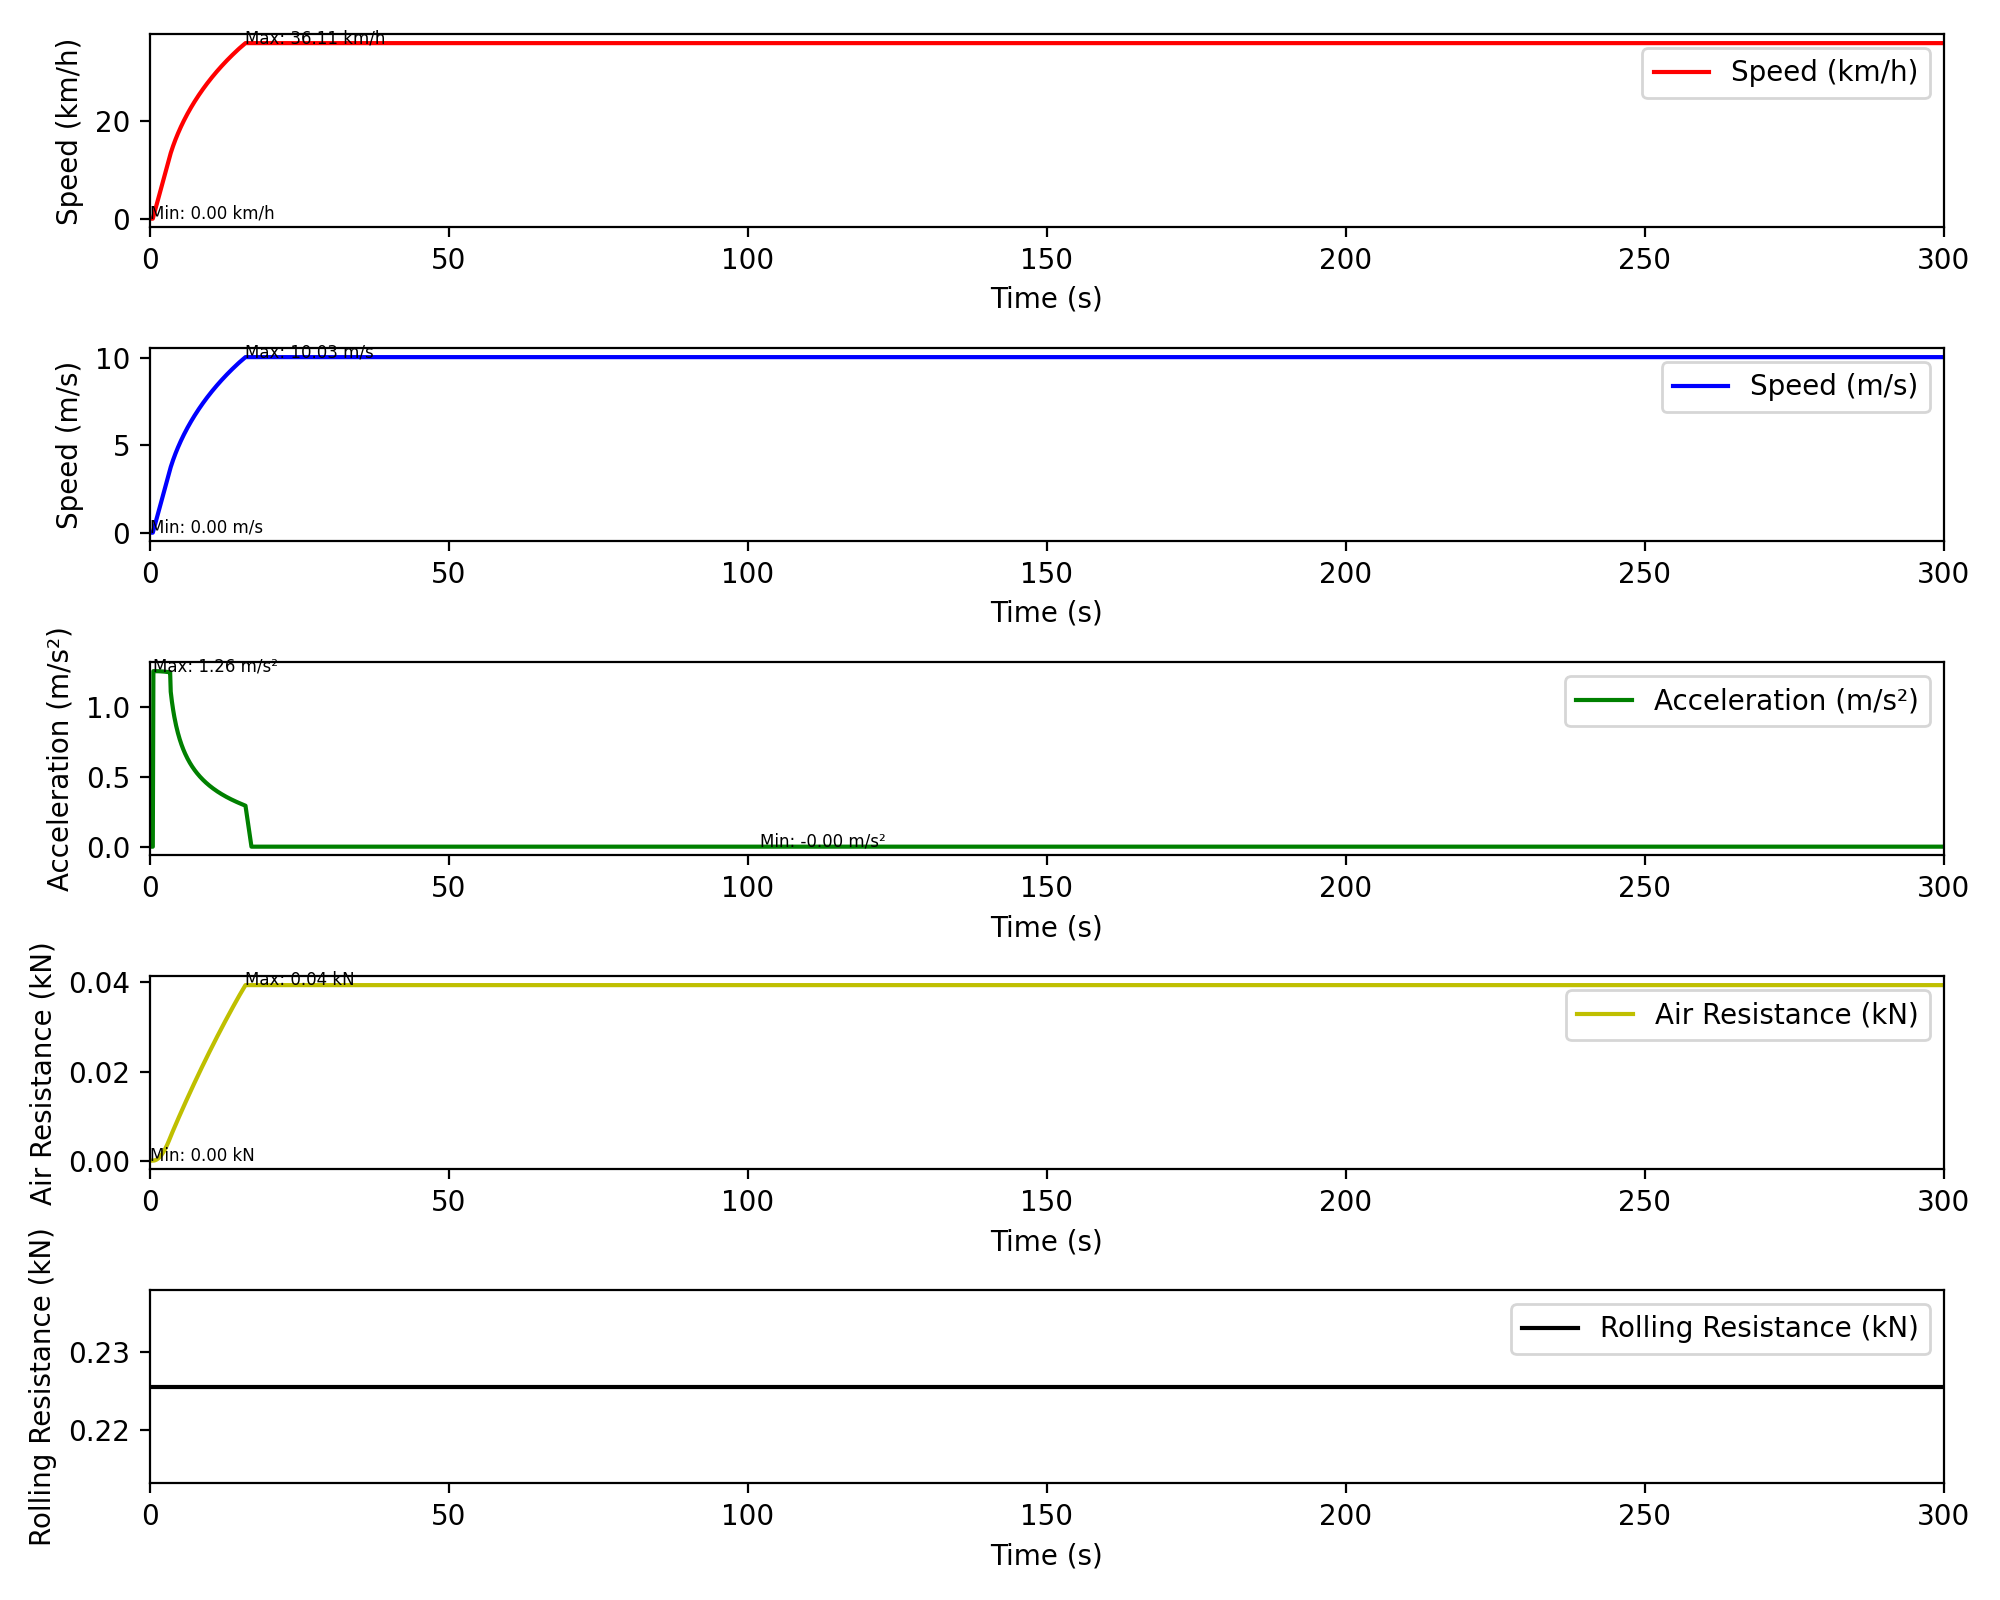
\includegraphics[width=0.87\linewidth]{E:/07. Master_Degree_ITC+UGA/02. ENES3_SGB_UGA/02. New Technology/PEMFC/Question_A_130_V2.png}
	\caption{\small {Plots related to Speed, acceleration, air resistance, and Total Force over time}}
	\label{12}
\end{figure}

The speed and acceleration are the same from the pervious but there are some change on the air resistance, rolling resistance and climbing	resistance. 

\begin{itemize}
	\item For the Air resistance using Equation (\ref{eq1}), we got the result shown in the Figure (\ref{12}).
	\item The Rolling Resistance using Equation (\ref{eq2}), as the result we can write :
	\begin{equation}
		F_{rolling}(t) = 200kg\times9.81m/s^2\times0.0115\times \cos(0^\circ) = \textbf{225.4926 N}\label{eq13}
	\end{equation}
	\item The Climbing Resistance using Equation (\ref{eq3}), as the result we computed :
	\begin{equation}
		F_{climb}(t) = Mg\sin(\alpha) = 2000kg \times 9.81m/s^2 \times \sin(2^\circ) = \textbf{684.811 N} \label{eq14}
	\end{equation}
	\item The total Force or Motor Force determined by usig Equation (\ref{eq5}) and the result of the calculation displayed at the black curve shown that the maximum motor force is \textbf{3.43 kN}.
\end{itemize}


\begin{figure}[h]
	\centering 
	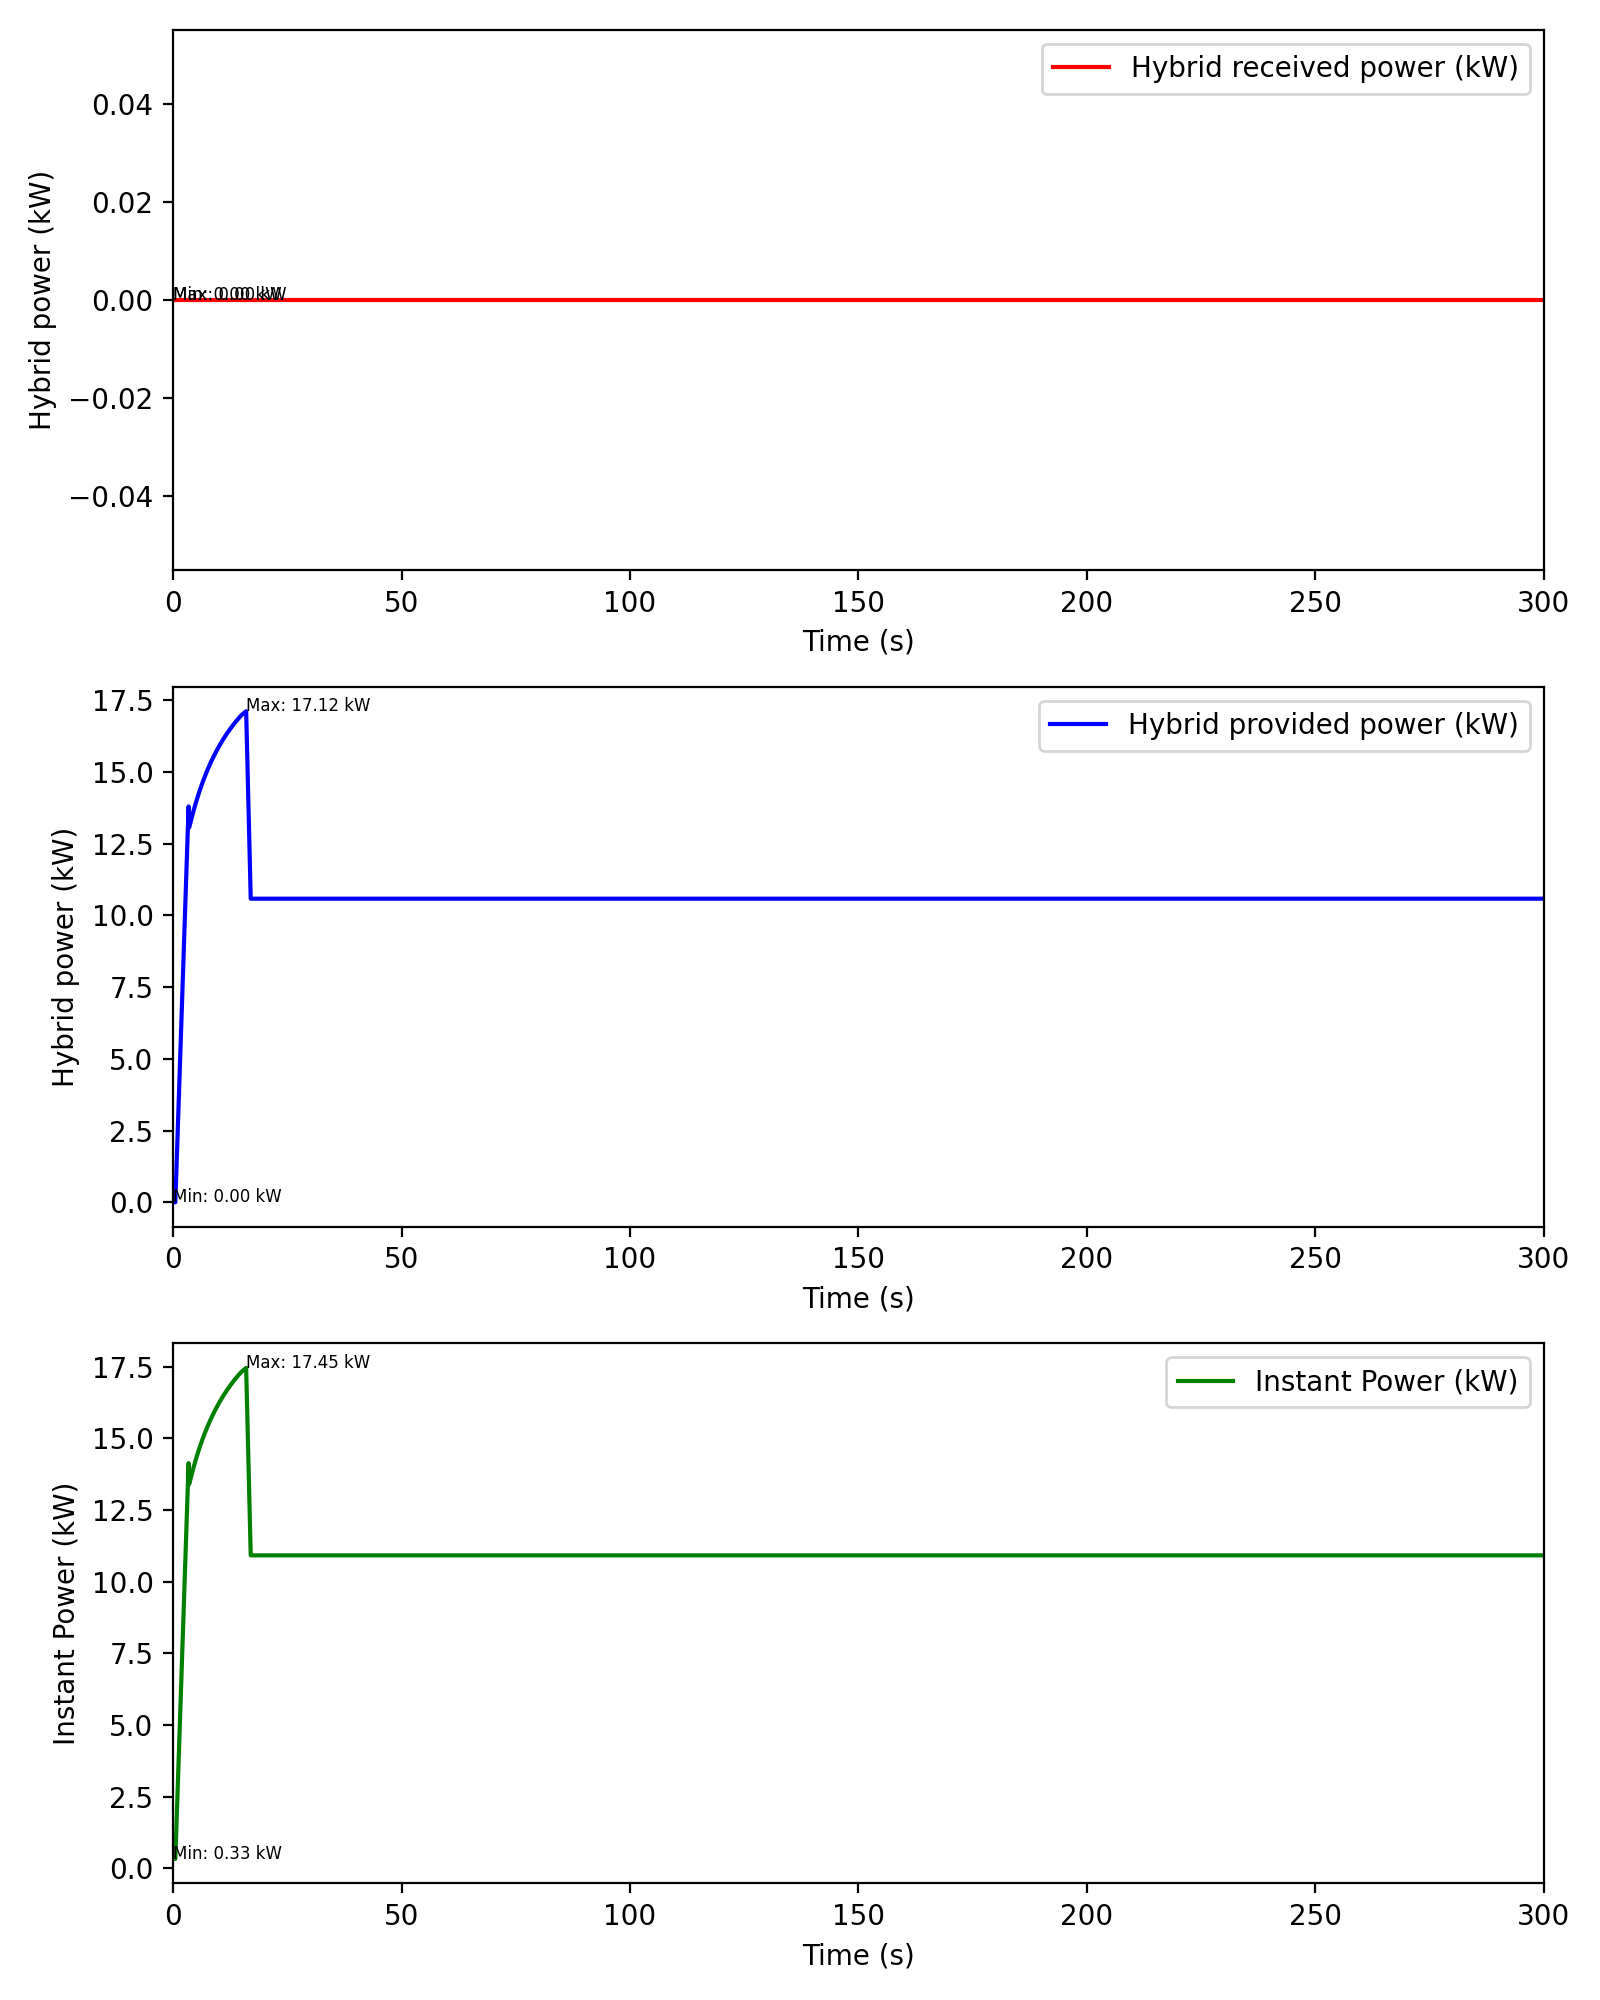
\includegraphics[width=0.83\linewidth]{E:/07. Master_Degree_ITC+UGA/02. ENES3_SGB_UGA/02. New Technology/PEMFC/Question_B_130_V2.png}
	\caption{\small {Hybrid working in Power transfer in Vehicle 130kmh}}
	\label{13}
\end{figure}

As show in Figure (\ref{13}), we can assume that vehicle at this speed characteristic shown that the Hybrid system did not receive any power from the motor but it provided full power to the motor.

\begin{figure}[h]
	\centering 
	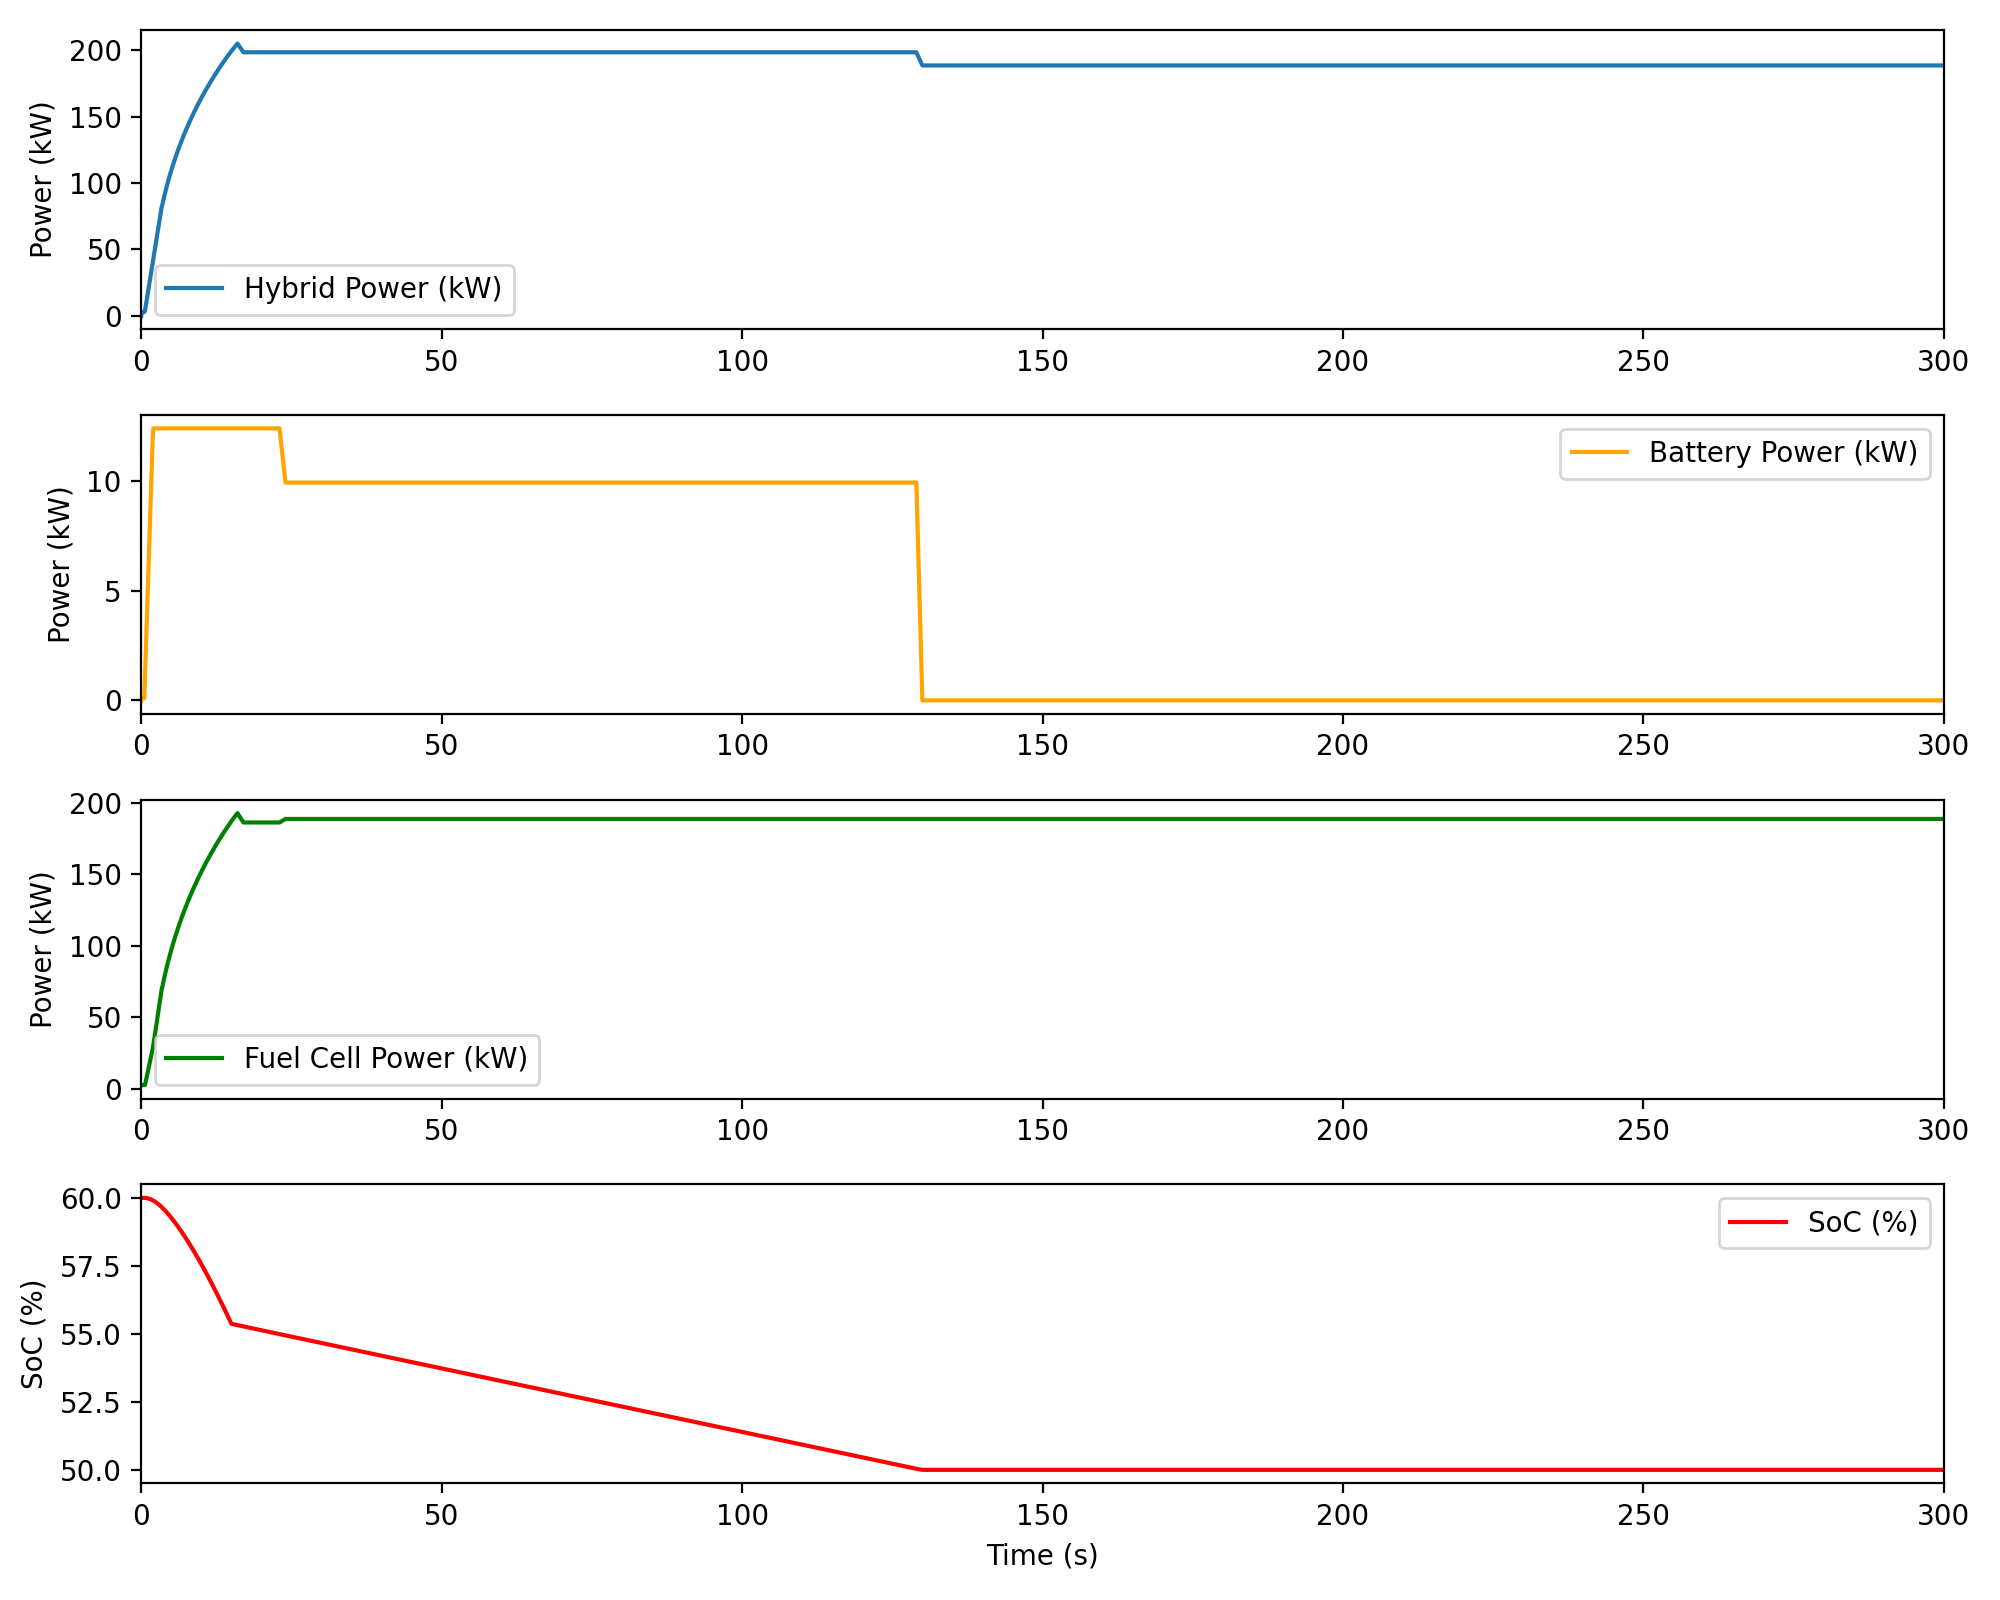
\includegraphics[width=0.95\linewidth]{E:/07. Master_Degree_ITC+UGA/02. ENES3_SGB_UGA/02. New Technology/PEMFC/Question_C_130_V2.png}
	\caption{\small {Hybrid working in Power transfer in Vehicle 130kmh}}
	\label{14}
\end{figure}

\begin{itemize}
	\item \textbf{Hybrid Power (kW) - Blue Curve (Top Plot):}
	\begin{itemize}
		\item The hybrid power increases sharply from 0 to about \textbf{17.45 kW} within the first few seconds.
		\item After this peak, the power stabilizes around \textbf{16 kW} and remains constant for the rest of the 300-second interval.
		\item This curve represents the total power output from the hybrid system.
	\end{itemize}
	
	\item \textbf{Battery Power (kW) - Orange Curve (Second Plot):}
	\begin{itemize}
		\item The battery power rises rapidly to a maximum value of \textbf{5.24 kW} at the beginning and then drops slightly, stabilizing around \textbf{4.5 kW}.
		\item The battery maintains this output throughout the time period shown.
		\item This shows the power contribution from the battery over time.
	\end{itemize}
	
	\item \textbf{Fuel Cell Power (kW) - Green Curve (Third Plot):}
	\begin{itemize}
		\item The fuel cell power ramps up initially to about \textbf{12.22 kW}.
		\item After reaching this maximum value, the fuel cell output drops slightly and stabilizes at around \textbf{10 kW} for the remainder of the time.
		\item This reflects the power contribution from the fuel cell system.
	\end{itemize}
	
	\item \textbf{State of Charge (SoC \%) - Red Curve (Bottom Plot):}
	\begin{itemize}
		\item The SoC starts at \textbf{60.0\%} and decreases gradually over time.
		\item By the end of the 300-second period, the SoC has dropped to \textbf{58.5\%}.
		\item This represents the decline in the battery's charge level over the duration of operation.
	\end{itemize}
\end{itemize}






%% =======================================1 . =========================================
% Sections and Subsections
\section{\underline{Analysis of the fuel cell system with WLTC profile}}

We assume that the fuel cell system of the vehicle has the following characteristics, based on some specifications of the Mirai 2 and an experimental study of the Mirai 1:

\begin{itemize}
	\item Hydrogen storage: 5.6 kg stored at 700 bars
	\item Molar mass of dihydrogen: 2.016 g/mol
	\item Enthalpy of hydrogen combustion in oxygen:
	\begin{itemize}
		\item LHV: 242 kJ/mol
		\item HHV: 285 kJ/mol
	\end{itemize}
	\item The hydrogen loss (mainly in the purge) represents 2\% of the consumed hydrogen
	\item Air stoichiometry is 1.5
	\item Atmospheric pressure is 1 bar
	\item Oxygen molar fraction in ambient air is 21\%
\end{itemize}

\begin{itemize}
	\item Air compressor's efficiency is 60\% (comprising both compression efficiency and electric motor efficiency)
	\item The air pressure inside the stack is variable, depending on the current density (data available in the file "BEfuelcellsystem.xlsx")
	\item The parasitic power consumed by the system auxiliaries depends on the stack current (data available in the file "BEfuelcellsystem.xlsx")
	\item The stack is composed of 330 cells of 273 cm\(^2\)
	\item The cell polarization curve has been studied during the vehicle operation. A simplified version is given below (data available in the file "BEfuelcellsystem.xlsx"):
\end{itemize}

\newpage


%% ======================================= a . =========================================

\subsection{Calculate and Plot as a function of the stack current: }
\subsubsection{The electrical power consumed by the air compressor}

To calculate of the compression power are proportional to the current:
\begin{equation}
	P_{comp}(t) = \frac{1}{\eta_{sys}(t)}q_{m_{air}(t)}c_pT_e(\tau^{\frac{\gamma-1}{\gamma}}-1)\label{eq2.1}
\end{equation}

Where we got :

\begin{itemize}
	\item Air mass Flow : 
		\begin{equation}
			q_{m_{air}}(t) = M_{air}F_{air}(t) = M_{air} \frac{v_{air}}{x_{O_2}}\frac{N_{cell}I(t)}{4\mathscr{F}} = M_{air} \frac{v_{air}}{x_{O_2}}\frac{P_{sys}(t)}{2v_{H_2}(t)\rho_{sys}\Delta H} 
			\label{eq2.2}
		\end{equation}
	\item Heat Capacity:
		\begin{equation}
			c_p =\frac{\gamma}{\gamma-1}\frac{R}{M} \label{eq2.3}
		\end{equation}
	\item Compression ratio:
		\begin{equation}
			\tau = \frac{\textit{p}_{out}}{\textit{p}_{in}} \label{eq2.4}
		\end{equation}
\end{itemize}

Get Equation (\ref{eq2.2}), Equation (\ref{eq2.3}), Equation (\ref{eq2.4}) Substitution into Equation (\ref{eq2.1})

\begin{equation}
	P_{comp}(t) = \frac{1}{\eta_{sys}(t)} \frac{v_{air}}{x_{O_2}}\frac{N_{cell}I(t)}{4\mathscr{F}} \frac{\gamma}{\gamma-1}RT_e(\tau^{\frac{\gamma-1}{\gamma}}-1)\label{eq2.1}
\end{equation}











\end{document} 